% Options for packages loaded elsewhere
\PassOptionsToPackage{unicode}{hyperref}
\PassOptionsToPackage{hyphens}{url}
\documentclass[
]{article}
\usepackage{xcolor}
\usepackage[margin=1in]{geometry}
\usepackage{amsmath,amssymb}
\setcounter{secnumdepth}{5}
\usepackage{iftex}
\ifPDFTeX
  \usepackage[T1]{fontenc}
  \usepackage[utf8]{inputenc}
  \usepackage{textcomp} % provide euro and other symbols
\else % if luatex or xetex
  \usepackage{unicode-math} % this also loads fontspec
  \defaultfontfeatures{Scale=MatchLowercase}
  \defaultfontfeatures[\rmfamily]{Ligatures=TeX,Scale=1}
\fi
\usepackage{lmodern}
\ifPDFTeX\else
  % xetex/luatex font selection
\fi
% Use upquote if available, for straight quotes in verbatim environments
\IfFileExists{upquote.sty}{\usepackage{upquote}}{}
\IfFileExists{microtype.sty}{% use microtype if available
  \usepackage[]{microtype}
  \UseMicrotypeSet[protrusion]{basicmath} % disable protrusion for tt fonts
}{}
\makeatletter
\@ifundefined{KOMAClassName}{% if non-KOMA class
  \IfFileExists{parskip.sty}{%
    \usepackage{parskip}
  }{% else
    \setlength{\parindent}{0pt}
    \setlength{\parskip}{6pt plus 2pt minus 1pt}}
}{% if KOMA class
  \KOMAoptions{parskip=half}}
\makeatother
\usepackage{longtable,booktabs,array}
\usepackage{calc} % for calculating minipage widths
% Correct order of tables after \paragraph or \subparagraph
\usepackage{etoolbox}
\makeatletter
\patchcmd\longtable{\par}{\if@noskipsec\mbox{}\fi\par}{}{}
\makeatother
% Allow footnotes in longtable head/foot
\IfFileExists{footnotehyper.sty}{\usepackage{footnotehyper}}{\usepackage{footnote}}
\makesavenoteenv{longtable}
\usepackage{graphicx}
\makeatletter
\newsavebox\pandoc@box
\newcommand*\pandocbounded[1]{% scales image to fit in text height/width
  \sbox\pandoc@box{#1}%
  \Gscale@div\@tempa{\textheight}{\dimexpr\ht\pandoc@box+\dp\pandoc@box\relax}%
  \Gscale@div\@tempb{\linewidth}{\wd\pandoc@box}%
  \ifdim\@tempb\p@<\@tempa\p@\let\@tempa\@tempb\fi% select the smaller of both
  \ifdim\@tempa\p@<\p@\scalebox{\@tempa}{\usebox\pandoc@box}%
  \else\usebox{\pandoc@box}%
  \fi%
}
% Set default figure placement to htbp
\def\fps@figure{htbp}
\makeatother
\setlength{\emergencystretch}{3em} % prevent overfull lines
\providecommand{\tightlist}{%
  \setlength{\itemsep}{0pt}\setlength{\parskip}{0pt}}
\usepackage{geometry}
\geometry{margin=1in}
\usepackage{pdflscape}
\newcommand{\blandscape}{\begin{landscape}}
\newcommand{\elandscape}{\end{landscape}}
\usepackage{bookmark}
\IfFileExists{xurl.sty}{\usepackage{xurl}}{} % add URL line breaks if available
\urlstyle{same}
\hypersetup{
  pdftitle={Preliminary 2026 assessment for eastern Bering Sea snow crab},
  pdfauthor={Grant Adams},
  hidelinks,
  pdfcreator={LaTeX via pandoc}}

\title{Preliminary 2026 assessment for eastern Bering Sea snow crab}
\author{Grant Adams}
\date{May 2026}

\begin{document}
\maketitle

{
\setcounter{tocdepth}{2}
\tableofcontents
}
\section{A. Executive summary}\label{a.-executive-summary}

This document is a preliminary stock assessment for eastern Bering Sea (EBS) snow crab (\emph{Chionoecetes opilio}) prepared for the May 2026 Crab Plan Team (CPT) meeting. Its purpose is to present model explorations requested by the SSC and CPT in 2025 and to seek guidance on which models to advance to the September 2026 final assessment cycle.

The 2026 cycle focused on three axes of uncertainty: (1) the influence of \emph{Chionoecetes} hybrids (snow \(\times\) Tanner crab) on assessment estimates when included in the survey and/or fishery data; (2) the impact of an updated maturity workflow developed by the Kodiak lab (Ryznar, in prep) that produces a spatiotemporally smoothed probability of terminal molt at size; and (3) attempts to improve model convergence (a bimodal jitter pattern was observed in the September 2025 assessment) using an updated plus group, a corrected total-male composition input, and/or the addition of an immature survey index.

A total of 14 models are presented. Across the candidate models, point estimates of the directed Tier 3 OFL ranged from approximately 36 to 56 thousand tonnes (kt), with the magnitude driven primarily by whether the immature survey index was included (which had a larger influence on the the scale of \(B_{MSY}\) and target \(F\)), whether hybrid catch was added to the directed pot fishery, and whether the new maturity workflow (which has a much weaker temporal trend in the probability of terminal molt at size) was used to specify the time-varying maturity ogive. The status of the stock relative to \(B_{MSY}\) in the candidate models was generally between 0.87 and 1.02. No author preferred model or final OFL is recommended at this time -- additional diagnostics, retrospective analyses, and Tier 4 calculations are recommended prior to the September document.

The most important result is that the bimodality observed in the 2025 jitter analysis (two clouds of converged models with directed OFLs differing by \textasciitilde5,000 t) does not persist when the immature survey index is included alongside the updated plus group. However, the immature index version of the model produces a much smaller \(B_{MSY}\) proxy and a substantially higher mature male natural mortality that warrants further investigation before September.

\section{B. Comments, responses and assessment summary}\label{b.-comments-responses-and-assessment-summary}

\subsection{SSC and CPT comments + author responses from June 2025}\label{ssc-and-cpt-comments-author-responses-from-june-2025}

\emph{2025(6) SSC. The maximin analysis should be completed assuming a Ricker stock-recruitment relationship, but including the same compensation ratios as the original Clark (1991) analysis.}

The Ricker curves (Figure 1) used in Clark were implemented in the maximin analysis presented last cycle (and now published in Fisheries Research: Szuwalski and Punt (2025) ``Spawning-biomass-per-recruit proxies for fisheries reference points under multiple axes of uncertainty''). Incorporating these into the analysis shifted the SPBR\% from \textasciitilde36\% to \textasciitilde34\% (Figure 2).

\emph{2025(6) SSC. As the figures presented on the updated 1991+ catch data appear to indicate substantial differences in male discards, the SSC requests that the September document more clearly describe changes in the discard estimation and accounting process.}

A presentation from January 2025 from ADFG (available on the council website) noted that the largest changes occurred for total catch through implementing consistent data filtering, expansion using directed pot lifts, and adjustments to biological strata. This process now allows for the production of a data file with all years of available data for each assessment cycle, rather than single years at a time which were appended to an existing data file. An apparent shift upwards in discards of males from the directed fishery results primarily from a change in when discard mortality is applied (before input into the data file {[}before 2025{]} or within the assessment code itself {[}after 2025{]}).

\emph{2025(6) SSC. Given the findings described in Mullowney and Baker (2021) from Canadian research indicating that the molt to maturity may occur at smaller sizes when lower densities of large males are present, it would be useful to determine if there is evidence for the same process occurring in EBS snow crab, and whether fishing mortality on the large males is consistently high enough to result in a strong effect. Further, it would be useful to evaluate whether clutch fullness may be related to size at maturity or the abundance of large-sized crab.}

\emph{Given that natural mortality events seem to switch among years and sexes depending on the model or input data, it would be prudent to investigate whether it is possible to estimate a direct link between natural mortality and a bottom temperature covariate of appropriate spatial and temporal scale.}

A manuscript describing both of these relationships for Bering Sea snow crab was presented in May/June 2024 (Figure 3; ``Density dependence can modulate climate change impacts on populations'') and was published in 2026 (Szuwalski et al., 2026). In that manuscript, warmer temperatures were associated with elevated mortality and higher densities of large males were associated with lower probabilities of terminally molting at
size.

The SSC responded to this presentation with the following text: ``The SSC emphasizes that projections of climate change impacts, while useful, are highly uncertain and. . . caution should be used when presenting
these results.''

Clutch fullness does not appear to be related to the abundance of large-size crab based on analyses in ``Spatial depletion rates in the eastern Bering Sea snow crab fishery'' (also presented in May 2024 and now in review for external publication). It is unclear if there is any relationship between clutch fullness and recruitment, though preliminary analyses suggest clutch fullness is not an important covariate for predicting recruitment strength.

These analyses come with the caveat that the Kodiak lab is revising their methods for analyzing the maturity data for snow crab.

\emph{2025(6) SSC. To explore development of an ABC control rule, the SSC requests that a yield per recruit analysis be developed for snow crab.}

Time did not allow for this exercise.

\emph{2024(10) SSC. SSC recommends standardizing the approach to the Tier 4 fallback across BBRKC, Tanner and snow crab assessments so that the same methods are used for each including all mature male biomass, a BMSY proxy based on the time-series of REMA-smoothed survey estimates and an FMSY proxy based on the best estimate of natural mortality (from the Tier 3 model). As the SSC intends the Tier 4 calculation only as a fallback if the Tier 3 analysis fails to converge, no other Tier 4 calculations need to be included in future assessments.}

In the 2025 document, Tier 4 HCRs were applied to rema-smoothed survey biomass estimates of three different size ranges: morphometrically mature males, large males (\textgreater=95mm), and preferred males (\textgreater101mm). The target biomass was set as the average of the time series from 1982-2024 and the target fishing mortality was set as 0.27, the median of the prior on natural mortality used in the integrated assessment. No kink exists in this harvest control rule. The resulting OFLs were 28.41 kt, 8.64 kt, and 6.11 kt for morphometric, large, and preferred males, respectively.

\emph{2024(10) SSC. The SSC highlighted that more research is needed on the basic reproductive biology of snow crab, specifically addressing the question of whether small males can and do mate with large females and produce progeny that will be large males under the right environmental conditions. The SSC strongly supports the proposed collaborative research to explore in situ observations of mating crab using a camera sled.}

We agree and no new research has been conducted within this timeframe.

\emph{2024(10) SSC. The highest priority would be to continue to refine the Maximin analysis as requested by the SSC in June 2024, specially using values of steepness of 0.50, 0.67, and 0.80, and considering both the Beverton-Holt and Ricker stock recruitment relationships. The yield analysis also indicated that fishing mortality rates much lower than F35\% achieved a high percentage of MSY, indicating potential flexibility in specifying reference points. The SSC suggested that some type of collaborative work during the spring, perhaps including SSC members and/or others might facilitate additional progress on this topic. The SSC is interested in developing a wider range of options for reference points for snow crab for consideration in the next assessment cycle.}

The analysis was not extended beyond what was presented in appendix A of the 2024 SAFE and would be of limited use until we know more about reproductive contribution of large male snow crab. The specific values for steepness noted by the SSC are arbitrary and do not match observations, estimates, or available data on the reproductive dynamics of snow crab. Until then, we know that the fishery will not exist without large males and we know that the large males are at historical lows, so we should focus our efforts on understanding the dynamics of large males.

\emph{2024(10) SSC. The SSC again requests an analysis of the probability of maturing/terminal molt which addresses the observation error in these data and the lack of a monotonically increasing curve. A hierarchical analysis that treats years as random effects might be a starting point. The SSC would also like to better understand the sampling design for the molt data and is concerned about the weighting of the spatial samples in the analysis; weighting should be based on abundance if the sampling rate differs by area (which it would, unless abundance were uniform and/or the targets were in direct proportion to abundance).}

The Kodiak lab gave a presentation describing how these data are analyzed. Potential changes to this workflow produces different values for the probability of having undergone terminal molt. Two models runs are included within the 2025 preliminary assessment and the current document to explore the impact of different assumptions about the probability of terminal molt.

\emph{2024(10) SSC. Investigate whether there is information outside the assessment model (e.g., larval or post-settlement data) or in the model, supporting estimated skewed sex-ratios at recruitment and the mismatch between recent large recruitments for males and females occurring in different years. Explore whether the estimated large differences in male and female recruitment years could be related to the lack of fit to molt-increment data.}

No new information has come to light on why this might be the case. Previous discussion centered around the possibility that different spatial distributions by sex of small crab could expose them to different environments, which could alter what we perceive as recruitment five years after settlement. While this difference is an interesting scientific question to pursue, solving it will not address the central problem in management: commercially preferred males are at historic lows over the last decade. Removing the females from the model entirely might be a prudent step towards focusing on the most pressing management problem at hand given conflicting trends.

\emph{2024(10) SSC. Geostatistical (e.g.~VAST) modeling of trawl survey data including both the NBS and EBS should be prioritized. This could help understand some of the inconsistent recruitment/growth trends observed in recent years as well as prepare for potential changes in stock distribution or productivity under future warming of the Bering Sea. Geostatistical modeling should evaluate alternative error distributions and other model configurations as appropriate.}

The Kodiak lab presented indices for mature females and large males in the 2025 May CPT.

\emph{2024(6) CPT. Tier 4 fallback - CPT supports: The author suggested an alternative for snow crab to the basic Tier 4 calculation that is being brought forward for other stocks. Specifically, a fallback Tier 4 option would be calculated as the vulnerable biomass in this year's survey (not smoothed, and vulnerable defined by a cutoff of 95 mm CW), decremented by the proportion of natural mortality that occurs between the time of the survey and the fishery, and M applied as the proxy for FMSY to calculate the Tier 4 OFL. The motivations identified for using the annual survey design-based estimate of vulnerable biomass rather than a REMA smooth through the survey time series were: 1) that the high number of positive stations for snow crab on survey (238 stations in 2023) make the design-based estimate a robust measure of annual biomass; and 2) that the large interannual fluctuations in biomass observed in some recent years would be poorly captured by a smooth. The motivation for decrementing the biomass estimate by the proportion of natural mortality occurring between the survey and the fishery is that failing to account for this mortality could lead to unintentionally high values of F if the Tier 4 fallback was used.}

No response.

\emph{2024(6) SSC. Concerning the GMACS assessment model, the SSC continues to recommend that the assessment author explore ways to incorporate the molt to maturity data in the model in a way that reflects the observation error associated with those estimates. An analysis in a GLMM modeling framework, which treats years as random effects, would provide smoother estimates, accommodate differing sample sizes by year and length, and deal appropriately with years in which data are missing. Another possibility that was suggested in the CPT report was to include the annual observed probabilities of terminal molt as data and then fit them, as in the Tanner crab assessment.}

The observation error is not considered when preparing the data that enters the assessment, so it is hard to understand how trying to consider uncertainty in the model that doesn't exist in the input data will provide meaningful results. I will try to do a better job of explaining this in my presentations. This is not to say there is no uncertainty in the probability of undergoing terminal molt, only that it is a less pressing problem than identifying appropriate reference points for snow crab.

\emph{2024(6) SSC. The SSC recommends that this model be brought forward in the fall but requests that an additional Tier 4 model be provided for comparison, as recommended in the Simpler Modeling Workshop report and requested in the SSC's June 2023 and October 2023 Reports. This additional model would use the random effects model (REMA) to smooth survey estimates and would not decrement with natural mortality.}

This is included in 2024 SAFE document.

\newpage

\section{C. Assessment scenarios}\label{c.-assessment-scenarios}

\subsection{Model summaries}\label{model-summaries}

The key assumptions of these models include:

\begin{itemize}
\item
  the probability of terminally molting at size varies over time and size and is specified based on observations from the survey data
\item
  survey selectivity is estimated by era (1982-88; 1989-present) and sex as a non-parametric curve subject to priors based on the BSFRF survey efficiency experiment data
\item
  growth is a linear function of pre-molt carapace width with a specified variability around post-molt size
\item
  all immature crab molt
\item
  natural mortality is estimated by sex and maturity state with additional mortality events estimated in 2018 and 2019 and subject to a prior based on an assumed longevity of 20 years
\item
  total and retained fishery selectivity are estimated logistic curves
\item
  all non-directed bycatch (e.g.~snow crab caught in the Tanner crab fishery or crab caught in the non-pelagic trawl fisheries) is lumped into a single `fishery' for which a single selectivity is estimated
\item
  recruitment is estimated separately for females and males and is allocated in the first 3 size bins
\end{itemize}

\subsection{Model scenarios}\label{model-scenarios}

A total of 14 models were explored. All models share the same structural assumptions described above and differ only in the version of GMACs, their data inputs, specification of the maturity ogive, and the definition of the plus group. The naming convention reflects an additive series of changes layered onto the September 2025 model (`25.1 gmacs').

The base (`rolled forward') model:

\begin{itemize}
\item
  \textbf{25.1 gmacs} -- the September 2025 author-recommended model, included for reference only. No data are updated and no structural changes are made.
\item
  \textbf{25.1 gmacs (update)} -- the September 2025 model using the updated version of GMACs (2.20.34; ** AEP **; Compiled 2026-01-15).
\end{itemize}

A series of incremental data and structural fixes:

\begin{itemize}
\tightlist
\item
  \textbf{25.1 gmacs (update + compfix)} -- as `update', but the total male composition data was updated to correct a small discrepancy between the file used in September 2025 and the version produced by the script.
\end{itemize}

@Cody, add why?

\begin{itemize}
\item
  \textbf{25.1 gmacs (update + plus group)} -- as `update', but the plus group is enlarged to include all crab greater than 135 mm carapace width (the previous model ignored all crab larger than 135 mm) for the retained male, total male, and discard female composition data. This model ran substantially faster (23 min, 9 sec) than the `update' model (29 min, 2 sec) and provides the basis for several of the sensitivities below.
\item
  \textbf{25.1 gmacs (update + imm\_surv + compfix)} and \textbf{25.1 gmacs (update + imm\_surv + plus group)} -- as `compfix' and `plus group', respectively, but with an immature survey index of biomass added. The immature index provides direct information on the abundance of immature crab and was found to remove the bimodality observed in jitter analyses (see Results).
\end{itemize}

Maturity scenarios:

\begin{itemize}
\tightlist
\item
  \textbf{25.1 gmacs (update + new\_mat)} -- as `update', but with the molting probability controls (the time- and size-varying probability of terminal molt) replaced with the array produced by the new maturity workflow developed by the Kodiak lab (E. Ryznar, in prep). The new workflow uses an \texttt{sdmTMB} spatiotemporal model fit to chela-based maturity classifications to produce a smoothed probability of being mature at size and location, integrated to a population-level annual ogive. The updated time series shows a much weaker temporal trend in the probability of terminal molt at intermediate sizes (e.g., at 77 mm) than the previous workflow. The updated maturity ogive resulted in differing time-series of mature male survey abundance and mature and immature male composition data. Note that the cv and sample size for both data sets were not adjusted.
\end{itemize}

@Cody, should immature time-series also vary? Should females also vary?

\begin{itemize}
\item
  \textbf{25.1 gmacs (update + new\_mat + compfix)} -- combination of the comp-fix and the new maturity workflow.
\item
  \textbf{25.1 gmacs (update + new\_mat + plus group)} -- combination of the plus group and the new maturity workflow.
\item
  \textbf{25.1 gmacs (update + new\_mat + imm\_surv + plus group)} -- combination of plus group, new maturity workflow, and the immature survey index.
\end{itemize}

Hybrid scenarios:

Hybrid catch and composition data were provided by ADF\&G (T. Jackson, ADF\&G Commercial Fisheries) as a separate species code lumped across opilio-type, bairdi-type, and unspecified hybrids; weights were calculated using snow crab length--weight parameters because the overwhelming majority of hybrids are of the opilio type. These data are \emph{additive} to the existing snow-crab time-series, except for retained catch which already contains hybrids landed under the snow-crab IFQ.

\begin{itemize}
\item
  \textbf{25.1 gmacs (update + hyb\_fishery)} -- the plus-group model with hybrids added to the directed-fishery composition and discard time-series. The CV on directed discards is held at 0.7. The retained male time-series uses is identical to the snow-crab retained file because retained catch already contains hybrids as they are not separately recorded. Observer non-directed bycatch is left unchanged.
\item
  \textbf{25.1 gmacs (update + hyb\_surv)} -- the plus-group model with hybrid catch and composition added to the NMFS summer trawl survey time-series and composition data.
\item
  \textbf{25.1 gmacs (update + hyb\_both)} -- combination of \texttt{hyb\_fishery} and \texttt{hyb\_surv}.
\item
  \textbf{25.1 gmacs (update + hyb\_both + new\_mat)} -- combination of \texttt{hyb\_both} and the new maturity workflow. Males snow crab and hybrids were apportioned to immature and mature using the new maturity ogive.
\end{itemize}

\section{D. Analytic approach}\label{d.-analytic-approach}

\subsection{Model description}\label{model-description}

The Generalized Model for Assessing Crustacean Stocks (GMACS) was adopted as the assessment platform for snow crab in 2022 after a demonstration that GMACS could effectively reproduce the dynamics of the status quo model and offered structural improvements. GMACS is an integrated, size-structured model developed using automatic differentiation software developed as a set of libraries under C++ (ADModel Builder). ADModel Builder can estimate a large number of parameters in a non-linear model using automatic differentiation software extended from Greiwank and Corliss (1991) and developed into C++ class libraries. GMACS version 2.20.34 was used for the author-preferred model after the January 2026 CPT.

The snow crab population dynamics model tracks the number of crab of sex \emph{s}, maturity state \emph{m}, during year \emph{y} at width \emph{w}, N\textsubscript{\emph{s,m,y,w}}. A terminal molt was modeled in which crab move from an immature to a mature state, after which no further molting occurred. The mid-points of the size bins tracked in the model spanned from 27.5 to 132.5 mm carapace width, with 5 mm size classes. For the author-preferred model, 407 parameters were estimated. Parameters estimated within the assessment included those associated with the population processes recruitment, growth, natural mortality (subject to an informative prior and two years of additional `mortality events' estimated in 2018 and 2019), fishing mortality, selectivity (fisheries and survey), and catchability. The yearly probability of undergoing terminal molt, weight at size, discard mortality, bycatch mortality, variance in growth increment, and parameters associated with proportion of recruitment allocated to size bin were estimated outside of the model or specified. See the GMACS repo linked at the end of this document to peruse the control files that specify the populations dynamics.

A `jittering' approach has been historically used to explore the impact of different starting values on the assessment output (Turnock, 2016). Jittering was implemented select both models with 2025 data. Parameter values were jittered based on a normal distribution centered on one with a standard deviation of 0.1 that was then translated to the parameter space defined by the initial value and its bounds.

\subsection{Model selection and evaluation}\label{model-selection-and-evaluation}

Models were evaluated based on their fit to the data, evidence of non-convergence, the credibility of the estimated population processes, and the strength of the influence of the assumptions of the model on the outcomes of the assessment. Note that for some of the model scenarios, data inputs are different and, therefore, model fits are not directly comparable.

\section{E. Results}\label{e.-results}

\subsubsection{Model convergence and comparison}\label{model-convergence-and-comparison}

All 14 models presented here produced small maximum gradients and Hessian matrices. As in past cycles, jittering was used to evaluate sensitivity to starting values: parameter values were jittered based on a normal distribution centered on one with a standard deviation of 0.1, translated to the parameter space defined by the initial value and its bounds. One hundred jitters were run for six models that span the range of structural and data choices -- `25.1 gmacs (update + plus group)', `25.1 gmacs (update + new\_mat + plus group)', `25.1 gmacs (update + hyb\_both)', `25.1 gmacs (update + hyb\_both + new\_mat)', `25.1 gmacs (update + imm\_surv + plus group)', and `25.1 gmacs (update + newmat + imm\_surv + plus group)'. Likelihood components by category for each candidate model are summarized in Table \ref{tab:like-comp-tot}.

The bimodality in management quantities reported in the 2025 preliminary and final assessments persists in most of the 2026 candidate models that do \emph{not} include the immature survey index, with two distinct clouds of converged OFLs separated by \textasciitilde50--100 negative-log-likelihood units and OFLs that differ by several thousand tonnes (Figure \ref{fig:jitter}). The bimodality is also visible in the corresponding estimates of 2024 male recruitment (Figure \ref{fig:jitt-rec}) and 2024 MMB (Figure \ref{fig:jitt-ssb}). Adding the immature survey index alongside the updated plus group (`25.1 gmacs (update + imm\_surv + plus group)') eliminates the bimodality entirely -- jitter runs converge to a single cloud of solutions (Figure \ref{fig:jitter}). This is an encouraging diagnostic, but the immature-index model also produces a substantially smaller \(B_{MSY}\) and a much higher mature male natural mortality (see below), so the apparent fix should not be interpreted as an unqualified improvement. The recent history of bimodality in this assessment (Turnock, 2016) suggests that resolving the underlying source of multiple optima will require further evaluation before September.

The `update' model continues to have difficulty fitting the terminal year of female biomass. Inputting a yearly varying probability of terminal molt from the new maturity workflow (`new\_mat' models) shifts the estimated population dynamics modestly but does not resolve the female terminal-year fit.

\subsubsection{Model fits}\label{model-fits}

Fits to the survey indices of mature biomass were broadly similar across the models (Figure \ref{fig:mmbfits}). The hybrid-survey models produce visibly higher predicted survey biomass in some years (the additional hybrid biomass is added to the snow-crab time-series), but the trend through time is unchanged. The models with the immature survey index (`imm\_surv') fit the new immature index well in recent years.

Fits to the non-directed fishery catches were good for all models (Figure \ref{fig:catchfits}). Fits to the directed-fishery retained catch were also good across the model set. Fits to the directed-fishery discard time-series differ in the hybrid-fishery models because the observed discards in those models include hybrid crab (and so are larger; e.g., \textasciitilde18 kt of legal-male hybrid catch in 1997 reported by ADF\&G with the caveat that observer hybrid identification quality decreases further back in the time-series; Table \ref{tab:obscatch}). The models accommodate the additional discards primarily through changes in estimated discard fishing mortality rather than through major changes in selectivity.

Differences among models in the fits to size composition data for retained catch in the directed fishery are small (size composition figures, below). Fits to the total size composition data from the directed fishery differ noticeably between the standard and the hybrid-fishery models, particularly for the larger size bins where hybrids are most prevalent. No visually discernible differences among models existed for female discards from the directed fishery. Fits to the non-directed fishery had some of the largest misfits of all data sources (particularly for male data), but this is unsurprising given a single estimated selectivity curve and changes in fishery behavior over time.

Fits to the survey size composition data were broadly similar across models in most years (size composition figures, below). The plus-group change (extending the plus group to all crab \textgreater{} 135 mm) makes a small visual difference for retained males but improves the runtime of the model substantially. All models had difficulty fitting the size composition data for mature males immediately after the early-1990s collapse, which could suggest some unmodelled size-based mortality. Fits to the mean growth data are shown in Figure \ref{fig:growthfits}.

\subsubsection{Estimated population processes}\label{estimated-population-processes}

The estimated abundance of commercially preferred male crab (\textgreater=101 mm carapace width) varied among models (Figure \ref{fig:obs-101-vs-pred}). The early years during which differences in survey selectivity occurred were particularly different. All models agreed that the abundance in recent years has been the lowest in the time series. The estimates of the most recent era of survey selectivity were similar across models for both sexes (Figure \ref{fig:select-prior}).

Estimated fisheries selectivities were similar across models (Figure \ref{fig:predselectfish}). Estimated fully-selected fishing mortality for the directed fishery was highly variable and relatively high for most of the fishery history (Figure \ref{fig:predfmort}). The total fishery selectivity curve is shifted far to the right, so only the largest crab experience the fully-selected fishing mortality. The probability of undergoing terminal molt is input as data (Figure \ref{fig:predmat}); the standard workflow produces a strong increasing trend through time at intermediate sizes (e.g., at 77 mm the probability rose from \textasciitilde0.2 in the early 1990s to \textasciitilde0.5 after 2010), while the new maturity workflow produces a much weaker temporal trend (\textasciitilde0.35--0.45 throughout the time series). The new workflow uses a spatiotemporal \texttt{sdmTMB} model fit to chela-based maturity classifications and borrows strength across years and locations for size bins with sparse chela data; it does not extrapolate the predicted spatial probability surface beyond stations with measured crab.

Trends in recruitment were very similar across models for the early time series, with some variability in scale and differences in timing between the sexes (Figure \ref{fig:recruits}). Differences in estimated recruitment in the most recent years were observed among models for males and contribute to differences in OFLs across the model set.

Base estimates of natural mortality for mature animals of both sexes were broadly similar across models, with one important exception: the model with the immature survey index produces a substantially higher mature male natural mortality than the other models (Figure \ref{fig:nat-m}). All models estimated additional mortality events that removed at least 80\% of crab by sex and maturity state (except for mature females) at some point during the marine heatwave of 2018--19. Models 25.1 gmacs and 25.1 gmacs (update + hyb\_both) estimated immature female natural mortality to above 100 in 2019, much higher than the other models and suggesting the models should not be selected to provide management advice.

\subsubsection{MMB and management quantities}\label{mmb-and-management-quantities}

Estimated mature male biomass time series had similar trends across models but the scales differed by up to \textasciitilde50\% in some years (Figure \ref{fig:predmmb}). Total numbers of crab predicted by the author-preferred model are reported in Table \ref{tab:predtotnum}. Estimates of \(B_{MSY}\), current MMB relative to \(B_{MSY}\), \(F_{MSY}\), \(F_{OFL}\), and the directed Tier 3 OFL are summarized in Table \ref{tab:stepchange}. Across models other than the immature-index sensitivity, \(B_{MSY}\) ranged from \textasciitilde160 to \textasciitilde184 kt and the directed OFL ranged from \textasciitilde42 to \textasciitilde56 kt, with current MMB at 87--102\% of \(B_{MSY}\). The immature-index plus-group model produced an outlier \(B_{MSY}\) of 94 kt and an OFL of \textasciitilde36 kt despite achieving a similar status; this large difference results from the much larger estimated mature male natural mortality in that model, which propagates into the spawning biomass-per-recruit reference points.

The hybrid-fishery and hybrid-both models produced slightly lower \(B_{MSY}\) proxies (\textasciitilde166--170 kt) than the corresponding non-hybrid models (\textasciitilde178--184 kt), reflecting the additional fishing mortality implied by the larger discard time-series. The new-maturity models produced \(B_{MSY}\) proxies near the lower end of the non-hybrid range (\textasciitilde172 kt) but the highest OFLs (\textasciitilde50--52 kt) because the weaker time trend in the probability of terminal molt translates into more crab being available at the size bins targeted by the fishery in the projection window.

\section{F. Calculation of the OFL}\label{f.-calculation-of-the-ofl}

\subsection{Methodology for OFL}\label{methodology-for-ofl}

\subsubsection{Tier 3}\label{tier-3}

Historically, the tier 3 OFL was calculated using proxies for biomass and fishing mortality reference points and a sloped control rule. Proxies for biomass and fishing mortality reference points were calculated using spawning-biomass-per-recruit methods (e.g.~Clark, 1991). After fitting the assessment model to the data and estimating population parameters, the model was projected forward 100 years using the estimated parameters under no exploitation and constant recruitment to determine `unfished' mature male biomass-per-recruit. Projections were repeated in which the bisection method was used to identify a fishing mortality that reduced the mature male biomass-per-recruit to 35\% of the unfished level (i.e.~F\textsubscript{35\%} and B\textsubscript{35\%}). Calculations of F\textsubscript{\emph{35\%}} were made under the assumption that bycatch fishing mortality was equal to the estimated average value over the last 10 years.

Calculated values of F\textsubscript{35\%} and B\textsubscript{35\%} were used in conjunction with a Tier 3 control rule to adjust the proportion of F\textsubscript{35\%} that is applied to the stock based on the status of the population relative to B\textsubscript{35\%} (Amendment 24, NMFS). To determine the F\textsubscript{OFL}, the population is projected to the time of fishing for the upcoming fishery under no fishing. If the MMB at that time exceeds 25\% of B\textsubscript{35\%}, a fishery can occur and the F\textsubscript{OFL} is calculated as:

\[\begin{equation}
F_{OFL} =
\begin{cases}
Bycatch  & if \frac{MMB}{B_{35}} \leq 0.25 \\[3ex]
\frac {F_{35} ( \frac {MMB}{B_{35}} - \alpha)}{1-\alpha}  & if 0.25 < \frac {MMB}{B_{35}} < 1 \\[3ex]
F_{35} & if MMB > B_{35}
\end{cases}
\end{equation}\]

Where MMB is the projected morphometrically mature male biomass in the current survey year after fishing at the F\textsubscript{\emph{OFL}}, B\textsubscript{\emph{35\%}} is the mature male biomass at the time of mating resulting from fishing at F\textsubscript{\emph{35\%}}, F\textsubscript{\emph{35\%}} is the fishing mortality that reduces the morphometrically mature male biomass per recruit to 35\% of unfished levels, and \(\alpha\) determines the slope of the descending limb of the harvest control rule (set to 0.1 here).

In addition to the status quo tier 3 control rule, a variation in which \textgreater=95mm carapace width mature male biomass was used as the currency of management is presented here.

Calculated Tier 3 OFLs across the 14 candidate models ranged from approximately 36 to 56 kt. Differences in OFLs were a result of differences in estimated MMB and the currency used for MMB; the immature-survey-index sensitivity sat at the low end of the range and the new-maturity sensitivities sat at the high end.

\subsubsection{Tier 4}\label{tier-4}

A Tier 4 fallback was not recalculated for this preliminary cycle. For reference, the September 2025 assessment applied Tier 4 HCRs to REMA-smoothed survey biomass estimates of three size ranges: morphometrically mature males, large males (\textgreater=95mm), and preferred males (\textgreater101mm), with the target biomass set as the 1982-2024 average and target fishing mortality set as 0.27 (the median of the prior on natural mortality). The resulting 2025 OFLs were 28.41 kt, 8.64 kt, and 6.11 kt for morphometric, large, and preferred males, respectively. An updated Tier 4 calculation following the standardized Tier 4 fallback recommended by the October 2024 SSC will be presented in the September 2026 document for whichever Tier 3 model is preferred.

\section{G. Calculation of the ABC}\label{g.-calculation-of-the-abc}

The recommended acceptable biological catch (ABC) is calculated by subtracting a 20\% buffer from the OFL to account for scientific uncertainty.

The buffers for the last six years used by the SSC were: 25\% (2025), 65\% (2024), 50\% (2023), (October 2022 SSC reports are not available online), 25\% (2021), and 25\% (2020).

\newpage

\subsection{Author recommendations}\label{author-recommendations}

This document is preliminary and no author-recommended OFL is presented. The author requests CPT and SSC guidance on which subset of the 14 candidate models to advance to the September 2026 final assessment cycle. Specifically, the author requests guidance on:

\begin{enumerate}
\def\labelenumi{\arabic{enumi}.}
\item
  \textbf{The plus-group structural change.} The updated plus group at \textgreater135 mm runs substantially faster, makes the size-composition fits at the largest sizes more interpretable, and does not appreciably change management quantities. The author suggests adopting this as the new structural baseline for September.
\item
  \textbf{Inclusion of an immature survey index.} Adding the index resolves the bimodality observed in jitters but produces a much larger mature male natural mortality. Before September the author intends to investigate whether the higher M is biologically credible (e.g., consistent with the mortality events implied by the 2018--19 marine heatwave) or whether it reflects model misspecification trying to reconcile the new index with the existing data. The author is also aprehensive to make model selection choices based on derived reference points.
\item
  \textbf{The new maturity workflow.} The Kodiak lab's spatiotemporal \texttt{sdmTMB}-based workflow produces a time series with a much weaker temporal trend in the probability of terminal molt at intermediate sizes than the legacy workflow. The author has no strong basis for preferring one workflow over the other at this time and requests CPT/SSC guidance on whether to adopt the new workflow as the default input.
\item
  \textbf{Hybrid treatment.} The author presents three hybrid sensitivities (fishery only, survey only, and both) layered onto the plus-group base. Including hybrids reduces \(B_{MSY}\) slightly and changes the directed OFL by a few thousand tonnes. ADF\&G has flagged that hybrid identification quality decreases in the older portions of the time series (notably the 1997--98 period when reported hybrid catches were very large) and that ADF\&G and NMFS do not currently use identical hybrid identification criteria. The author recommends that a snow crab only and hybrid (survey and fishery) models be adopted moving forward.
\end{enumerate}

For September the author plans to: (a) finalize the plus-group structural change; (b) develop a Tier 4 fallback for whichever Tier 3 model is preferred; (c) investigate the inclusion of the immature survey index; and (d) complete retrospective analyses for the recommended models.

\section{H. Data gaps and research priorities}\label{h.-data-gaps-and-research-priorities}

Several data and structural issues identified during the May 2026 cycle warrant follow-up:

\begin{itemize}
\item
  \textbf{Hybrid identification consistency between ADF\&G and NMFS.} ADF\&G classifies hybrid crab into three categories (opilio-type, bairdi-type, and unspecified) using a hybrid identification key based on eye color, epistome shape, and secondary morphological characteristics. ADF\&G and NMFS do not currently agree on the number of secondary characteristics required for a positive hybrid identification, and the unspecified-hybrid category are present in a non-trivial portion of the time series. Resolving identification criteria across agencies and propagating the resulting categorization back through the historical observer time series would improve the hybrid-data products available to the assessment. However, the value add to the snow crab assessment may be minimal given the low percentage of opilio-type hybrids in the data.
\item
  \textbf{Apportionment of retained catch between snow crab and hybrids.} Hybrids are currently retained under either the snow-crab or the Tanner-crab IFQ depending on regulatory identification but are not separately tracked in the retained-catch data. ADF\&G has indicated it does not yet have a method for partitioning historical retained catch into hybrid versus parent species. Developing such a partitioning would allow the hybrid sensitivity to be explored more fully (presently the retained time-series is identical between the hybrid and non-hybrid models because retained catch already contains hybrids).
\item
  \textbf{Quality control on early hybrid catch estimates.} The ADF\&G hybrid total-catch estimates contain unexpectedly large values in 1997 (\textasciitilde18 kt of legal-male hybrid catch) and 1998 (\textasciitilde15 kt), with high-CPUE pots peppered around the fishery footprint rather than concentrated in obvious hot spots. ADF\&G has flagged these years as requiring follow-up before the data should be considered reliable for regular assessment use.
\item
  \textbf{Maturity workflow comparison.} The new spatiotemporal maturity workflow produces a much weaker temporal trend in the probability of terminal molt at size than the legacy workflow. Side-by-side documentation of the two workflows, an evaluation of the spatial sample sizes of chela measurements (which are sparse at many stations and many sizes), uncertainty, and quantification of the degrees of freedom consumed by the spatial process would help the CPT and SSC evaluate the two approaches.
\item
  \textbf{Source of bimodality in the snow crab assessment.} Although the immature survey index appears to remove the bimodal jitter signal in the May 2026 candidate models, the underlying source of multiple optima is not understood. A focused investigation of which parameter combinations produce the two clouds (e.g., recruitment in the most recent years, \(M\) events, or selectivity parameters) would help clarify whether the immature index is solving a real problem or is masking it.
\item
  \textbf{Reproductive biology of large male snow crab.} As noted in 2024 and 2025 SSC comments, more research is needed on whether small males can and do mate with large females and produce progeny that will be large males under favorable environmental conditions. This question remains the main axis of uncertainty because the fishery cannot exist without large males and large males are at historical lows.
\end{itemize}

\section{I. Supplemental information}\label{i.-supplemental-information}

Input and output for the models described here can be found at \url{https://github.com/szuwalski/snow_crab/tree/dev-Grant}.

The new maturity workflow can be found at \url{https://github.com/eryznar/Chionoecetes.maturity.workflow}.

GMACS code and documentation can be found at: \url{https://github.com/GMACS-project}.

\newpage

\section{J. References}\label{j.-references}

Chilton, E.A., C.E. Armisted and R.J. Foy. 2009. Report to industry on the 2009 Eastern Bering Sea crab survey. AFSC Processed Report 2009-XX.

Clark, W.G. 1991. Groundfish exploitation rates based on life history parameters. Can. J. fish. Aquat. Sci. 48: 734-750.

Conan, G.Y. and Comeau, M. 1986. Functional maturity and terminal molt of male snow crab. Can J. Fish Aqaut Sci. 43(9):

Dawe, E.G., D.M. Taylor, J.M. Hoenig, W.G. Warren, and G.P. Ennis. 1991. A critical look at the idea of terminal molt in male snow crab (Chionoecetes opilio). Can. J. Fish. Aquat. Sci. 48: 2266-2275.

Ennis, G.P., Hooper, R.G. Taylor, D.M. 1988. functional maturity in smalle male snow crab. Can J Fish Aquat Sci. 45(12):

Ernst, B, J.M.(Lobo) Orensanz and D.A. Armstrong. 2005. Spatial dynamics of female snow crab (Chionoecetes opilio) in the eastern Bering Sea. Can. J. Fish. Aquat. Sci. 62: 250-268.

Fonseca, D. B., B. Sainte-Marie, and F. Hazel. 2008. Longevity and change in shell condition of adult male snow crab Chionoecetes opilio inferred from dactyl wear and mark-recapture data. Transactions of the American Fisheries Society 137:1029-1043.

Fournier, D.A. and C.P. Archibald. 1982. A general theory for analyzing catch-at-age data. Can.J.Fish.Aquat.Sci. 39:1195-1207.

Greiwank, A. and G.F. Corliss(eds). 1991. Automatic differentiation of algorithms: theory, implementation and application. Proceedings of the SIAM Workshop on the Automatic Differentiation of Algorithms, held Jan.~6-8, Breckenridge, CO. Soc. Indust. And Applied Mathematics, Philadelphia.

Hamel, O. 2015. A method for calculating a meta-analytical prior for the natural mortality rate using multiple life history correlates. ICES Journal of Marine Science. 72: 62-69.

Hoenig, J. 1983. Empirical use of longevity data to estimate mortality rates. Fish. Bull. 82: 898-903.

Lang, C. A., J. I. Richar, and R. J. Foy. 2019. The 2018 eastern Bering Sea continental shelf and northern Bering Sea trawl surveys: Results for commercial crab species. U.S. Dep. Commer., NOAA Tech. Memo. NMFS-AFSC-386, 220 p.

McAllister, M.K. and Ianelli, J.N. 1997. Bayesian stock assessment using catch-at-age data and the sampling importance resampling algorithm. Can. J. Fish. Aquat. Sci. 54(2): 284-300.

Mcbride (1982). Tanner crab tag development and tagging experiments 1978-1982. In Proceedings of the International Symposium of the Genus Chionoecetes. Lowell Wakefield Fish. Symp. Ser., Alaska Sea Grant Rep.~82-10. University of Alaska, Fairbanks, Alaska. Pp. 383-403.

Methot, R. D. 1990. Synthesis model: An adaptable framework for analysis of diverse stock assessment data. Int. N. Pac. Fish. Comm. Bull. 50:259-277.

Murphy, J.T. Rugolo, L.J., Turnock, B.J. 2018. Estimation of annual, time-varying natural mortality and survival for Eastern Bering Sea snow crab (Chionoecetes opilio) with state-space population models. Fish Res 205: 122-131.

Murphy, J.T. Rugolo, L.J., Turnock, B.J. 2017. Integrating demographic and environmental variables to calculate an egg production index for the Eastern Bering Sea snow crab (Chionoecetes opilio). Fisheries Research. 193: 143-157.

Murphy, J. T., A. B. Hollowed, J. J. Anderson. 2010. Snow crab spatial distributions: examination of density-dependent and independent processes. Pp. 49-79. In G. Kruse, G. Eckert, R. Foy, G. Kruse, R. Lipcius, B. St.~Marie, D. Stram, D. Woodby (Eds.), Biology and management of Exploited Crab Populations Under Climate Change. Alaska Sea Grant Program Report AK-SG-10-01, University of Alaska Fairbanks, AK. \url{Doi:10.4027/bmecppc.2010.19}

Myers, R.A. 1998. When do environment-recruitment correlations work? Reviews in Fish Biology and Fisheries. 8(3): 285-305.

Nevissi, A.E., J.M. Orensanz, A.J.Paul, and D.A. Armstrong. 1995. Radiometric Estimation of shell age in Tanner Crab, Chionoecetes opilio and C. bairdi, from the eastern Bering Sea, and its use to interpret indices of shell age/condition. Presented at the International symposium on biology, management and economics of crab from high latitude habitats October 11-13, 1995, Anchorage, Alaska.

NPFMC (North Pacific Fishery Management Council). 2007. Environmental Assessment for Amendment 24. Overfishing definitions for Bering Sea and Aleutian Islands King and Tanner crab stocks. North Pacific Fishery Management Council,Anchorage, AK, USA..

NPFMC (North Pacific Fishery Management Council). 2000. Bering Sea snow crab rebuilding plan. Amendment 14. Bering Sea Crab Plan Team, North Pacific Fishery Management Council,Anchorage, AK, USA..

NPFMC 1998. Bering Sea and Aleutian Islands Crab FMP. Bering Sea Crab Plan Team, North Pacific Fishery Management Council, P. O. Box 103136, Anchorage, Ak 99510.

Orensanz, J.M., J. Armstrong, D. Armstrong and R. Hilborn. 1998. Crustacean resources are vulnerable to serial depletion - the multifaceted decline of crab and shrimp fisheries in the Greater Gulf of Alaska. Reviews in Fish Biology and Fisheries 8:117-176.

Otto, R.S. 1998. Assessment of the eastern Bering Sea snow crab, Chionoecetes opilio, stock under the terminal molting hypothesis. In Proceedings of the North Pacific Symposium on Invertebrate Stock Assessment and Management. Edited by G.S. Jamieson and A. Campbell. Can. Spec. Publ. Fish. Aquat. Sci. 125. pp.~109-124.

Parada, C., Armstrong, D.A., Ernst, B., Hinckley, S., and Orensanz, J.M. 2010. Spatial dynamics of snow crab (Chionoecetes opilio) in the eastern Bering Sea--Putting together the pieces of the puzzle. Bulletin of Marine Science. 86(2): 413-437.

Paul, A.J., J.M. Paul and W.E. Donaldson. 1995. Shell condition and breeding success in Tanner crab. Journal of Crustacean Biology 15: 476-480.

Restrepo, V.R, G.G. Thompson, P.M. Mace, W.L. Gabriel, L.L. Low, A.D. MacCall, R.D. Methot, J E. Powers, B.L. Taylor, P.R. Wade, and J.F. Witzig. 1998. Technical guidance on the use of precautionary approaches to implementing National Standard 1 of the Magnuson-Stevens Fishery Conservation and Management Act. NOAA Technical Memorandum NMFS-F/SPO-31.

Rugolo, L.J., D. Pengilly, R. MacIntosh and K. Gravel. 2005. Reproductive dynamics and life-history of snow crab (Chionoecetes opilio) in the eastern Bering Sea. Final Completion Report to the NOAA, Award NA17FW1274, Bering Sea Snow Crab Fishery Restoration Research.

Rodionov, S. 2004. A sequential algorithm for testing climate regime shifts. Geophysical Research Letters 21: L09204.

Sainte-Marie, B., Raymond, S., and Brethes, J. 1995. Growth and maturation of the male snow crab, Chionoecetes opilio (Brachyura: Majidae). Can.J.Fish.Aquat.Sci. 52:903-924.

Sainte-Marie, B., J. Sevigny and M. Carpentier. 2002. Interannual variability of sperm reserves and fecundity of primiparous females of the snow crab (Chionoecetes opilio) in relation to sex ratio. Can.J.Fish.Aquat.Sci. 59:1932-1940.

Somerton, D.A. and Otto, R.S. 1999. Net efficiency of a survey trawl for snow crab and Tanner crab. Fish Bull 97: 617-625.

Somerton, D.A. Weinberg, K.L., Goodman, S.E. 2013. Catchability of snow crab by the eastern Bering Sea bottom trawl survey estimated using a catch comparison experiment. Can.J.Fish.Aquat.Sci. 70: 1699-1708.

Szuwalski, C.S. 2022a. Stock assessment of Eastern Bering Sea snow crab. Stock Assessment and Fishery Evaluation Report for the King and Tanner Crab Fisheries of the Bering Sea and Aleutian Islands Regions. 2021 Crab SAFE. North Pacific Fishery Management Council,1007 West 3rd Ave., Suite 400, L92 Building, 4th floor. Anchorage, AK 99501

Szuwalski, C.S. 2021a. Stock assessment of Eastern Bering Sea snow crab. Stock Assessment and Fishery Evaluation Report for the King and Tanner Crab Fisheries of the Bering Sea and Aleutian Islands Regions. 2021 Crab SAFE. North Pacific Fishery Management Council,1007 West 3rd Ave., Suite 400, L92 Building, 4th floor. Anchorage, AK 99501

Szuwalski, C.S. 2021b. An exploration of assessment options for eastern Bering Sea snow crab that consider additional time-variation in population processes. North Pacific Fishery Management Council,1007 West 3rd Ave., Suite 400, L92 Building, 4th floor. Anchorage, AK 99501

Szuwalski, C.S. 2020a. Stock assessment of Eastern Bering Sea snow crab. Stock Assessment and Fishery Evaluation Report for the King and Tanner Crab Fisheries of the Bering Sea and Aleutian Islands Regions. 2021 Crab SAFE. North Pacific Fishery Management Council,1007 West 3rd Ave., Suite 400, L92 Building, 4th floor. Anchorage, AK 99501

Szuwalski, C.S., Cheng, W., Foy. R., Hermann. A.J., Hollowed, A.B., Holsman, K., Lee, J., Stockhausen, W., Zheng, J. 2020b. Climate change and the future productivity and distribution of crab in the eastern Bering Sea. ICES J. Mar.~Sci. 78(2): 502-515.

Szuwalski, C.S. 2019a. Stock assessment of Eastern Bering Sea snow crab. Stock Assessment and Fishery Evaluation Report for the King and Tanner Crab Fisheries of the Bering Sea and Aleutian Islands Regions. 2021 Crab SAFE. North Pacific Fishery Management Council,1007 West 3rd Ave., Suite 400, L92 Building, 4th floor. Anchorage, AK 99501

Szuwalski, C.S. 2019b. A summary of model runs requested by the CPT. North Pacific Fishery Management Council,1007 West 3rd Ave., Suite 400, L92 Building, 4th floor. Anchorage, AK 99501

Szuwalski, C.S. 2018a. Stock assessment of Eastern Bering Sea snow crab. Stock Assessment and Fishery Evaluation Report for the King and Tanner Crab Fisheries of the Bering Sea and Aleutian Islands Regions. 2021 Crab SAFE. North Pacific Fishery Management Council,1007 West 3rd Ave., Suite 400, L92 Building, 4th floor. Anchorage, AK 99501

Szuwalski, C.S. 2018b. A summary of model runs requested by the CPT. North Pacific Fishery Management Council,1007 West 3rd Ave., Suite 400, L92 Building, 4th floor. Anchorage, AK 99501

Szuwalski, C.S. 2017a. Stock assessment of Eastern Bering Sea snow crab. Stock Assessment and Fishery Evaluation Report for the King and Tanner Crab Fisheries of the Bering Sea and Aleutian Islands Regions. 2021 Crab SAFE. North Pacific Fishery Management Council,1007 West 3rd Ave., Suite 400, L92 Building, 4th floor. Anchorage, AK 99501

Szuwalski, C.S. and Punt, A.E. 2013. Regime shifts and recruitment dynamics of snow crab, Chionoecetes opilio, in the eastern Bering Sea. Fisheries Oceanography, 22: 345-354.

Szuwalski, C.S. and Punt, A.E. 2012. Fisheries management for regime-based ecosystems: a management strategy evaluation for the snow crab fishery in the eastern Bering Sea. ICES Journal of Marine Science. 70: 955-967.

Szuwalski, C.S. and Punt, A.E. 2025. Spawning-biomass-per-recruit proxies for fisheries reference points under multiple axes of uncertainty. Fisheries Research. 289: 107494.

Tamone, S.L., M. Adams and J.M. Dutton. 2005. Effect of eyestalk ablation on circulating ecdysteroids in hemolymph of snow crab Chionoecetes opilio: physiological evidence for a terminal molt. Integr. Comp. Biol., 45(120), p.166-171.

Then, A. Y., Hoenig, J. M., Hall, N. G., and Hewitt, D. A. 2015. Evaluating the predictive performance of empirical estimators of natural mortality rate using information on over 200 fish species. ICES Journal of Marine Science, 72: 82--92.

Turnock, B.J. 2016. Snow crab assessment model scenarios and convergence testing. Alaska Fishery Science Center.

watson, J. 1972. Mating behavior in the spider crab, Chionoecetes opilio. J Fish REs Boar Can 29: 447-449.

Zheng, J., S. Siddeek, D. Pengilly, and D. Woodby. 2002. Overview of recommended harvest strategy for snow crab in the Eastern Bering Sea. Regional Information Report No.~5J02-03. Alaska Department of Fish and Game. Juneau, Alaska.

Zheng, J., G.H. Kruse, and D.R. Ackley. 2001. Spatial distribution and recruitment patterns of snow crab in the eastern Bering Sea. Spatial Processes and management of marine populations. Alaska sea grant college program. AK-SG-01-02, 2001.

\newpage
\begin{landscape}

\begin{table}

\caption{\label{tab:like-comp-tot}\label{tab:like-comp-tot} Likelihood components by category and model.}
\centering
\begin{tabular}[t]{l|r|r|r|r|r|r|r|r|r|r|r|r|r|r}
\hline
  & 25.1 & u & u+imm+cf & u+imm+pg & u+cf & u+pg & u+nm+pg & u+nm+imm+pg & u+hs & u+hf & u+hb & u+nm & u+nm+cf & u+hb+nm\\
\hline
Catch & 363.29 & 372.63 & 320.69 & 336.81 & 376.61 & 372.48 & 375.39 & 446.42 & 365.61 & 901.75 & 900.71 & 373.01 & 375.90 & 948.57\\
\hline
Index & 133.91 & 153.18 & 186.97 & 192.22 & 153.13 & 142.26 & 136.07 & 392.17 & 150.66 & 155.98 & 157.41 & 145.56 & 147.62 & 158.77\\
\hline
Size & -28953.17 & -28974.26 & -28959.05 & -28984.14 & -28989.55 & -29004.09 & -29037.38 & -29035.29 & -28975.55 & -28945.08 & -28969.26 & -29012.56 & -29030.66 & -29037.24\\
\hline
SRR & 184.82 & 172.13 & 170.56 & 175.40 & 171.41 & 183.86 & 185.33 & 170.73 & 177.10 & 170.19 & 177.18 & 179.88 & 179.75 & 184.50\\
\hline
Tag & 7966.89 & 0.00 & 0.00 & 0.00 & 0.00 & 0.00 & 0.00 & 0.00 & 0.00 & 0.00 & 0.00 & 0.00 & 0.00 & 0.00\\
\hline
Penalties & 756.80 & 756.59 & 759.27 & 763.19 & 756.98 & 760.25 & 758.13 & 757.72 & 750.47 & 752.64 & 750.43 & 755.01 & 755.04 & 753.74\\
\hline
Priors & 379.40 & 386.20 & 433.03 & 431.91 & 392.27 & 386.44 & 390.01 & 434.01 & 363.64 & 384.95 & 366.69 & 391.09 & 392.36 & 383.36\\
\hline
Initial\_size\_structure & 0.00 & 0.00 & 0.00 & 0.00 & 0.00 & 0.00 & 0.00 & 0.00 & 0.00 & 0.00 & 0.00 & 0.00 & 0.00 & 0.00\\
\hline
Growth\_data & 0.00 & 7965.70 & 7964.95 & 7965.71 & 7965.87 & 7965.23 & 7969.97 & 7970.11 & 7965.74 & 7963.69 & 7963.67 & 7970.57 & 7970.54 & 7966.31\\
\hline
Positive\_growth\_penalty & 0.00 & 0.00 & 0.00 & 0.00 & 0.00 & 0.00 & 0.00 & 0.00 & 0.00 & 0.00 & 0.00 & 0.00 & 0.00 & 0.00\\
\hline
Total & -19168.06 & -19167.83 & -19123.58 & -19118.89 & -19173.27 & -19193.59 & -19222.49 & -18864.12 & -19202.34 & -18615.87 & -18653.17 & -19197.43 & -19209.45 & -18642.00\\
\hline
\end{tabular}
\end{table}

\end{landscape}

\newpage

\newpage

\begin{longtable}[]{@{}
  >{\raggedright\arraybackslash}p{(\linewidth - 12\tabcolsep) * \real{0.0897}}
  >{\raggedright\arraybackslash}p{(\linewidth - 12\tabcolsep) * \real{0.1410}}
  >{\raggedright\arraybackslash}p{(\linewidth - 12\tabcolsep) * \real{0.1923}}
  >{\raggedright\arraybackslash}p{(\linewidth - 12\tabcolsep) * \real{0.1410}}
  >{\raggedright\arraybackslash}p{(\linewidth - 12\tabcolsep) * \real{0.1667}}
  >{\raggedright\arraybackslash}p{(\linewidth - 12\tabcolsep) * \real{0.1282}}
  >{\raggedright\arraybackslash}p{(\linewidth - 12\tabcolsep) * \real{0.1410}}@{}}
\caption{\label{tab:obscatch} Comparison of observed retained catches, discards, and bycatch between base and hybrid cases (Units: 1,000 tonnes).}\tabularnewline
\toprule\noalign{}
\begin{minipage}[b]{\linewidth}\raggedright
Year
\end{minipage} & \begin{minipage}[b]{\linewidth}\raggedright
Retained
(kt)
\end{minipage} & \begin{minipage}[b]{\linewidth}\raggedright
Non-directed
Bycatch
\end{minipage} & \begin{minipage}[b]{\linewidth}\raggedright
Discard
Male Pot
\end{minipage} & \begin{minipage}[b]{\linewidth}\raggedright
Discard
Male Pot +
hybrids
\end{minipage} & \begin{minipage}[b]{\linewidth}\raggedright
Discard
Female
\end{minipage} & \begin{minipage}[b]{\linewidth}\raggedright
Discard
Female +
hybrids
\end{minipage} \\
\midrule\noalign{}
\endfirsthead
\toprule\noalign{}
\begin{minipage}[b]{\linewidth}\raggedright
Year
\end{minipage} & \begin{minipage}[b]{\linewidth}\raggedright
Retained
(kt)
\end{minipage} & \begin{minipage}[b]{\linewidth}\raggedright
Non-directed
Bycatch
\end{minipage} & \begin{minipage}[b]{\linewidth}\raggedright
Discard
Male Pot
\end{minipage} & \begin{minipage}[b]{\linewidth}\raggedright
Discard
Male Pot +
hybrids
\end{minipage} & \begin{minipage}[b]{\linewidth}\raggedright
Discard
Female
\end{minipage} & \begin{minipage}[b]{\linewidth}\raggedright
Discard
Female +
hybrids
\end{minipage} \\
\midrule\noalign{}
\endhead
\bottomrule\noalign{}
\endlastfoot
1982 & 11.85 & 0.37 & 1.27 & 1.27 & 0.02 & 0.02 \\
1983 & 12.16 & 0.47 & 1.24 & 1.24 & 0.01 & 0.01 \\
1984 & 29.94 & 0.5 & 2.76 & 2.76 & 0.01 & 0.01 \\
1985 & 44.45 & 0.43 & 4.01 & 4.01 & 0.01 & 0.01 \\
1986 & 46.22 & 0 & 4.25 & 4.25 & 0.02 & 0.02 \\
1987 & 61.4 & 0 & 5.52 & 5.52 & 0.03 & 0.03 \\
1988 & 67.79 & 0 & 5.82 & 5.82 & 0.04 & 0.04 \\
1989 & 73.33 & 0.1 & 6.68 & 6.68 & 0.05 & 0.05 \\
1990 & 149.1 & 0.33 & 35.55 & 42.15 & 1.52 & 1.54 \\
1991 & 143 & 4.45 & 9.03 & 15.25 & 0.2 & 0.23 \\
1992 & 104.7 & 2.05 & 21.18 & 26.96 & 0.28 & 0.29 \\
1993 & 67.94 & 1.13 & 22.27 & 22.87 & 0.12 & 0.12 \\
1994 & 34.16 & 0.7 & 7.78 & 8.08 & 0.08 & 0.08 \\
1995 & 29.8 & 1.04 & 14.73 & 16.54 & 0.02 & 0.03 \\
1996 & 54.24 & 1.22 & 23.23 & 27.49 & 0.1 & 0.11 \\
1997 & 110.4 & 0.73 & 7.1 & 26.23 & 0.1 & 0.12 \\
1998 & 88.15 & 0.58 & 19.5 & 14.64 & 0.01 & 0.02 \\
1999 & 15.1 & 0.24 & 4.13 & 5.32 & 0.01 & 0.01 \\
2000 & 11.46 & 0.25 & 3.25 & 4.03 & 0 & 0 \\
2001 & 14.8 & 0.18 & 3.98 & 6.64 & 0.02 & 0.02 \\
2002 & 12.84 & 0.1 & 4.5 & 4.75 & 0 & 0 \\
2003 & 10.86 & 0.14 & 2.4 & 0.08 & 0 & 0 \\
2004 & 11.29 & 0.18 & 3.58 & 3.83 & 0 & 0 \\
2005 & 16.77 & 0.19 & 0.62 & 0.73 & 0 & 0 \\
2006 & 16.49 & 0.36 & 4.17 & 4.24 & 0 & 0 \\
2007 & 28.59 & 0.31 & 5.77 & 5.81 & 0.02 & 0.02 \\
2008 & 26.56 & 0.19 & 5.11 & 5.33 & 0.02 & 0.02 \\
2009 & 21.78 & 0.39 & 4.28 & 4.39 & 0.01 & 0.01 \\
2010 & 24.61 & 0.14 & 4.47 & 4.61 & 0.01 & 0.01 \\
2011 & 40.29 & 0.14 & 3.73 & 3.88 & 0.19 & 0.19 \\
2012 & 30.05 & 0.15 & 5.53 & 5.7 & 0.06 & 0.06 \\
2013 & 24.49 & 0.16 & 10.61 & 10.72 & 0.12 & 0.12 \\
2014 & 30.82 & 0.62 & 11.62 & 11.94 & 0.3 & 0.3 \\
2015 & 18.42 & 1.58 & 10.9 & 11.02 & 0.12 & 0.12 \\
2016 & 9.78 & 0.04 & 4.51 & 4.7 & 0.03 & 0.03 \\
2017 & 8.6 & 0.1 & 5.88 & 5.95 & 0.03 & 0.03 \\
2018 & 12.51 & 0.4 & 8.63 & 8.62 & 0.02 & 0.02 \\
2019 & 15.43 & 0.21 & 15.61 & 15.61 & 0.02 & 0.02 \\
2020 & 20.41 & 0.19 & 6.12 & 6.12 & 0 & 0 \\
2021 & 2.52 & 0.13 & 1.68 & 1.68 & 0 & 0 \\
2022 & 0 & 0.06 & 0 & 0 & 0 & 0 \\
2023 & 0 & 0.11 & 0 & 0 & 0 & 0 \\
2024 & 2.15 & 0.09 & 0.66 & 0.67 & 0 & 0 \\
\end{longtable}

\newpage

\begin{landscape}

\begin{table}

\caption{\label{tab:stepchange}\label{tab:stepchange} Management quantities derived from maximum likelihood estimates by model using Tier 3 reference points. Reported natural mortality is for mature males, average recruitment is for males, and status and MMB were estimates for February 15 of the completed crab year.}
\centering
\begin{tabular}[t]{l|r|r|r|r|r}
\hline
Model & BMSY & Bcurr/BMSY & Fmsy & Fofl & OFL\\
\hline
25.1 & 173.12 & 0.89 & 34.78 & 30.49 & 37.72\\
\hline
u & 181.27 & 0.89 & 37.56 & 32.92 & 45.48\\
\hline
u+imm+cf & 94.33 & 0.95 & 157.51 & 149.34 & 36.42\\
\hline
u+imm+pg & 96.37 & 0.98 & 157.78 & 154.63 & 35.75\\
\hline
u+cf & 177.53 & 0.90 & 41.65 & 37.24 & 45.88\\
\hline
u+pg & 179.46 & 0.89 & 40.10 & 35.25 & 44.99\\
\hline
u+nm+pg & 177.61 & 0.94 & 38.44 & 35.86 & 50.29\\
\hline
u+nm+imm+pg & 166.67 & 0.91 & 75.48 & 68.21 & 60.01\\
\hline
u+hs & 176.33 & 0.93 & 34.46 & 31.59 & 47.83\\
\hline
u+hf & 169.34 & 0.91 & 37.04 & 33.39 & 44.16\\
\hline
u+hb & 168.16 & 0.95 & 35.31 & 33.46 & 42.25\\
\hline
u+nm & 171.92 & 0.97 & 38.16 & 36.80 & 51.40\\
\hline
u+nm+cf & 173.54 & 0.96 & 39.48 & 37.94 & 51.53\\
\hline
u+hb+nm & 169.75 & 1.01 & 44.15 & 44.15 & 49.57\\
\hline
\end{tabular}
\end{table}

\end{landscape}

\newpage

\newpage

\begin{longtable}[]{@{}
  >{\centering\arraybackslash}p{(\linewidth - 4\tabcolsep) * \real{0.1250}}
  >{\raggedright\arraybackslash}p{(\linewidth - 4\tabcolsep) * \real{0.1250}}
  >{\raggedright\arraybackslash}p{(\linewidth - 4\tabcolsep) * \real{0.1389}}@{}}
\caption{\label{tab:predtotnum} Maximum likelihood estimates of total numbers of crab (billions), not subject to survey selectivity at the time of the survey.}\tabularnewline
\toprule\noalign{}
\begin{minipage}[b]{\linewidth}\centering
~
\end{minipage} & \begin{minipage}[b]{\linewidth}\raggedright
Survey
year
\end{minipage} & \begin{minipage}[b]{\linewidth}\raggedright
Total
numbers
\end{minipage} \\
\midrule\noalign{}
\endfirsthead
\toprule\noalign{}
\begin{minipage}[b]{\linewidth}\centering
~
\end{minipage} & \begin{minipage}[b]{\linewidth}\raggedright
Survey
year
\end{minipage} & \begin{minipage}[b]{\linewidth}\raggedright
Total
numbers
\end{minipage} \\
\midrule\noalign{}
\endhead
\bottomrule\noalign{}
\endlastfoot
\textbf{2} & 1982 & 8.6 \\
\textbf{3} & 1983 & 11.39 \\
\textbf{4} & 1984 & 12.04 \\
\textbf{5} & 1985 & 17.74 \\
\textbf{6} & 1986 & 30.04 \\
\textbf{7} & 1987 & 26.91 \\
\textbf{8} & 1988 & 24.57 \\
\textbf{9} & 1989 & 17.89 \\
\textbf{10} & 1990 & 15.25 \\
\textbf{11} & 1991 & 15.59 \\
\textbf{12} & 1992 & 17.53 \\
\textbf{13} & 1993 & 14.49 \\
\textbf{14} & 1994 & 13.36 \\
\textbf{15} & 1995 & 10.85 \\
\textbf{16} & 1996 & 8.57 \\
\textbf{17} & 1997 & 9.27 \\
\textbf{18} & 1998 & 6.93 \\
\textbf{19} & 1999 & 6.79 \\
\textbf{20} & 2000 & 6.47 \\
\textbf{21} & 2001 & 5.1 \\
\textbf{22} & 2002 & 6.01 \\
\textbf{23} & 2003 & 17.11 \\
\textbf{24} & 2004 & 12.61 \\
\textbf{25} & 2005 & 11.25 \\
\textbf{26} & 2006 & 9.16 \\
\textbf{27} & 2007 & 7.15 \\
\textbf{28} & 2008 & 6.62 \\
\textbf{29} & 2009 & 18.98 \\
\textbf{30} & 2010 & 12.48 \\
\textbf{31} & 2011 & 9.61 \\
\textbf{32} & 2012 & 8.08 \\
\textbf{33} & 2013 & 9.09 \\
\textbf{34} & 2014 & 8.11 \\
\textbf{35} & 2015 & 18.56 \\
\textbf{36} & 2016 & 26.22 \\
\textbf{37} & 2017 & 32.19 \\
\textbf{38} & 2018 & 21.88 \\
\textbf{39} & 2019 & 11.88 \\
\textbf{40} & 2020 & 4.95 \\
\textbf{41} & 2021 & 6.65 \\
\textbf{42} & 2022 & 8.83 \\
\textbf{43} & 2023 & 15.9 \\
\textbf{44} & 2024 & 15.47 \\
\textbf{45} & 2025 & 12.75 \\
\end{longtable}

\newpage

\begin{figure}[H]
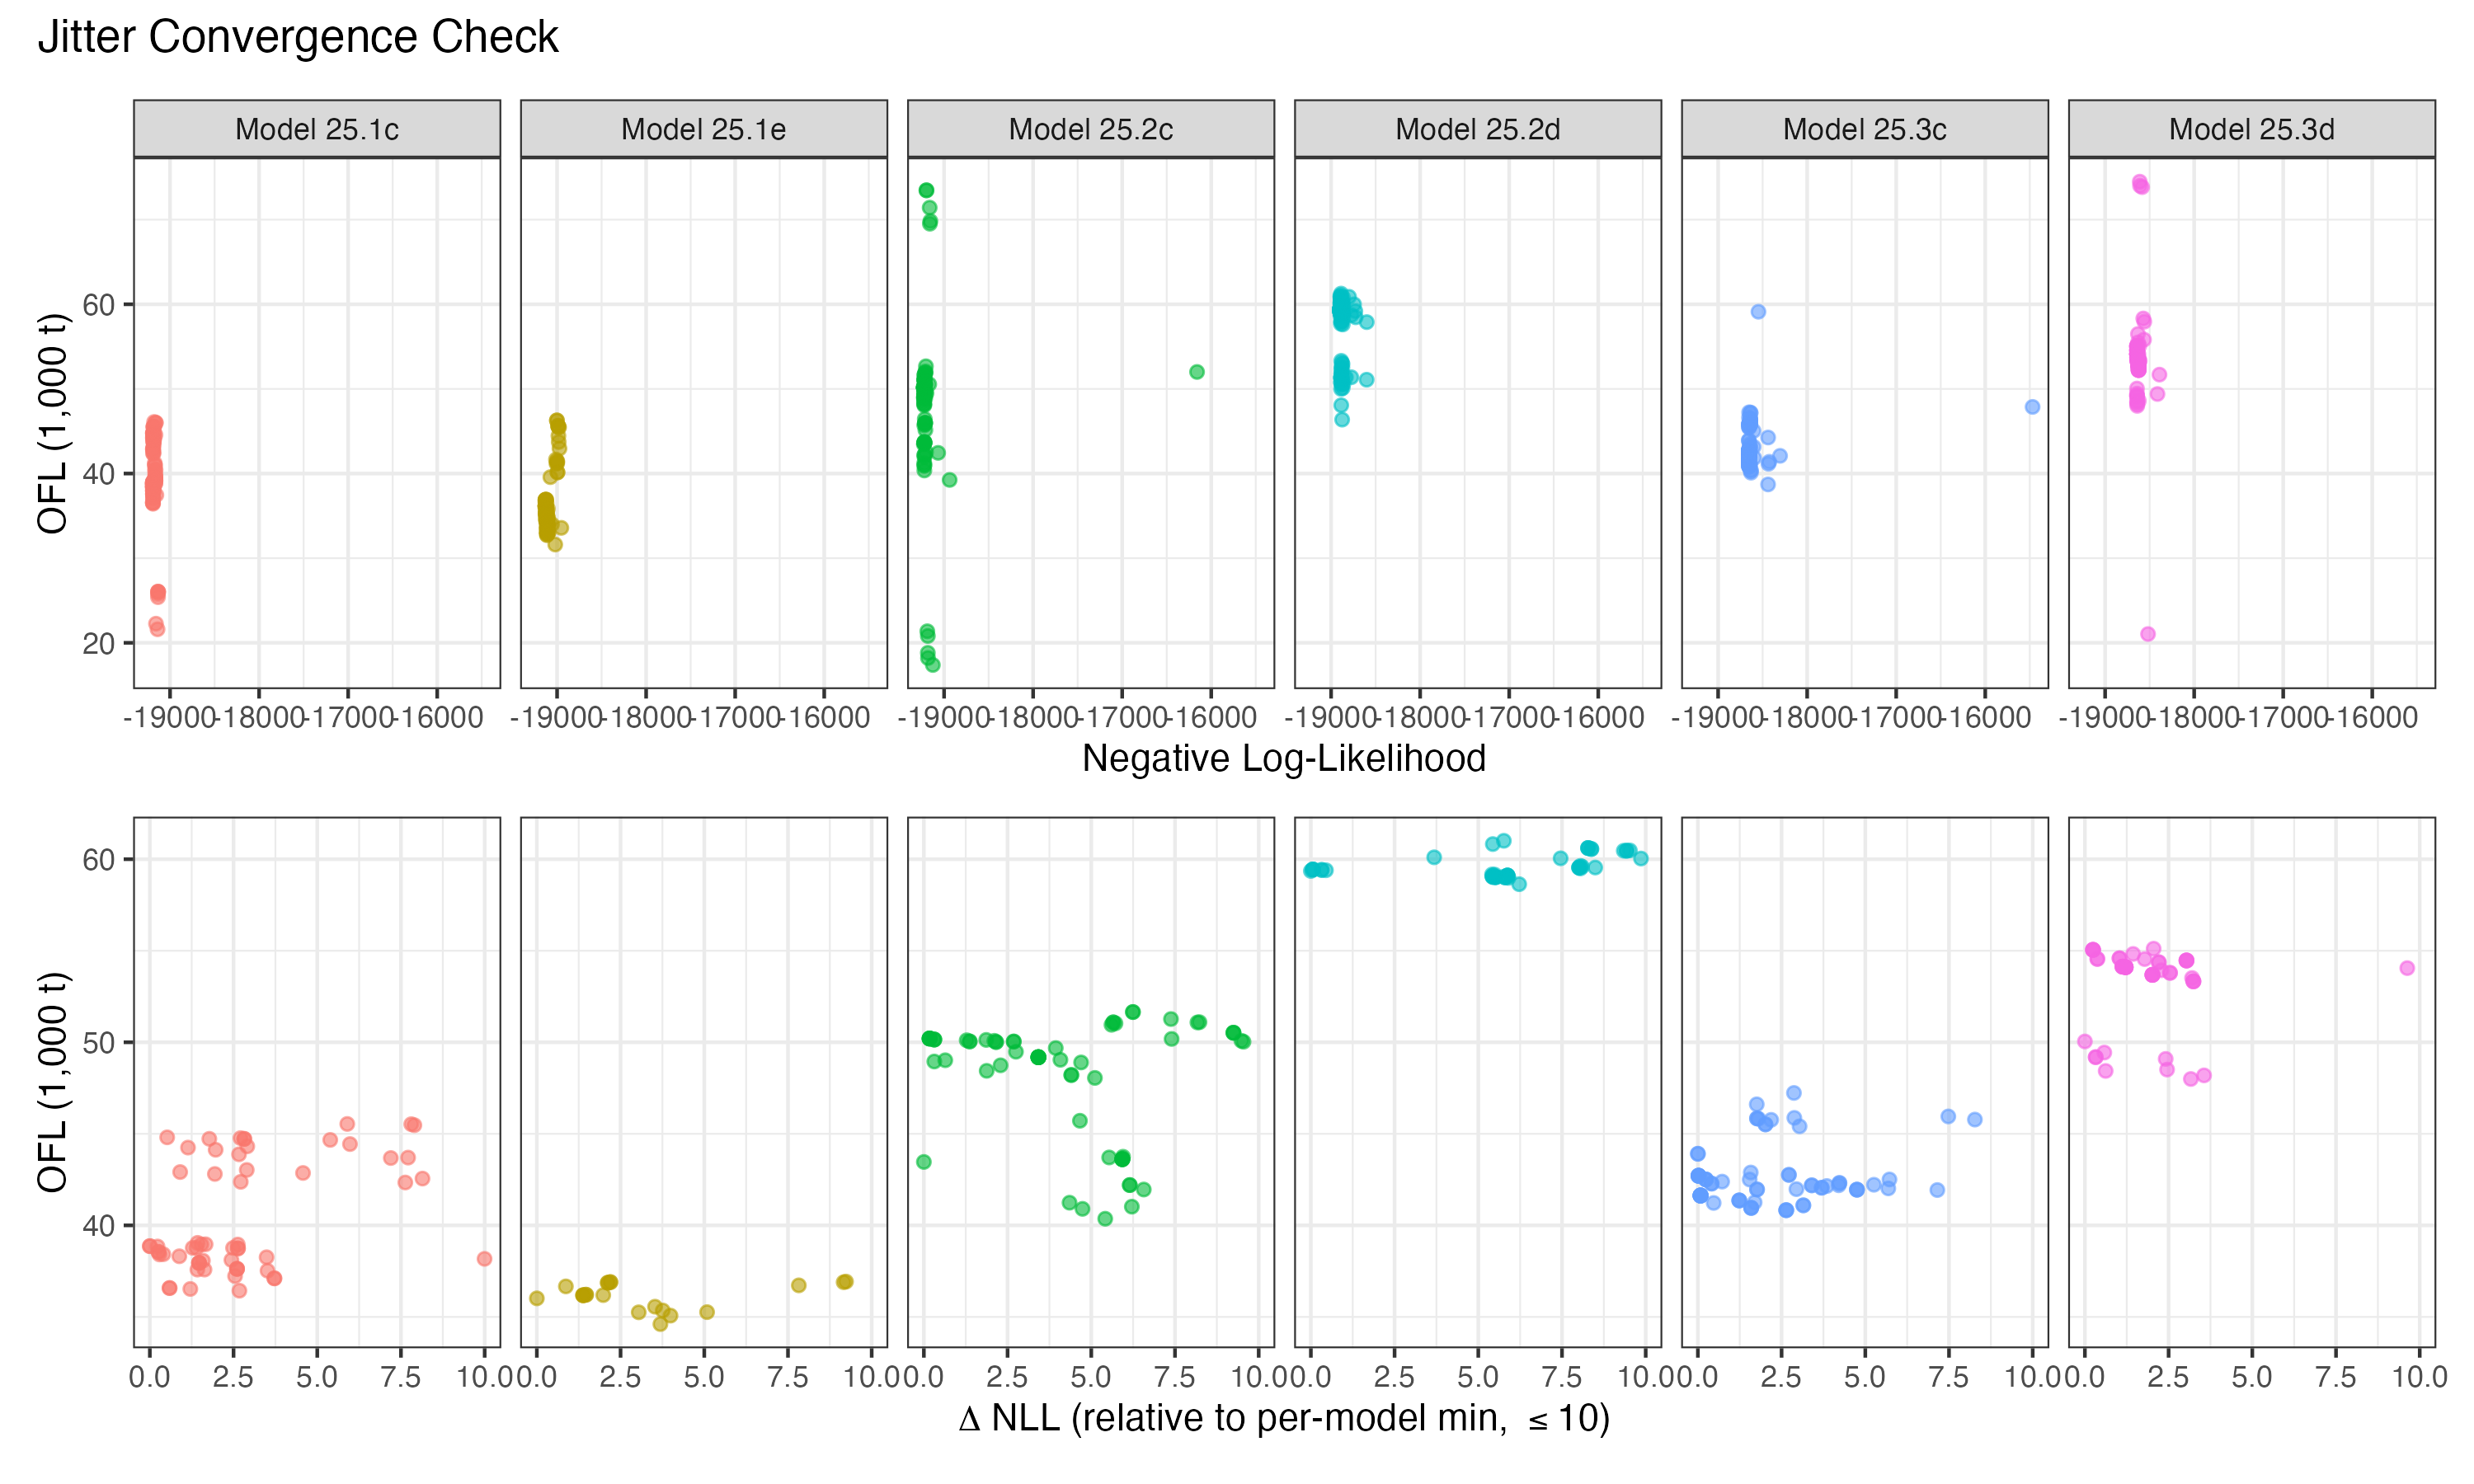
\includegraphics[width=1\linewidth]{plots/jittered_results_ofl} \caption{Directed OFLs resulting from 100 jitter runs for the models that span the structural and data choices presented in this document. Each point is a converged jitter run; clouds separated vertically reflect alternative local optima.}\label{fig:jitter}
\end{figure}

\newpage

\begin{figure}[H]
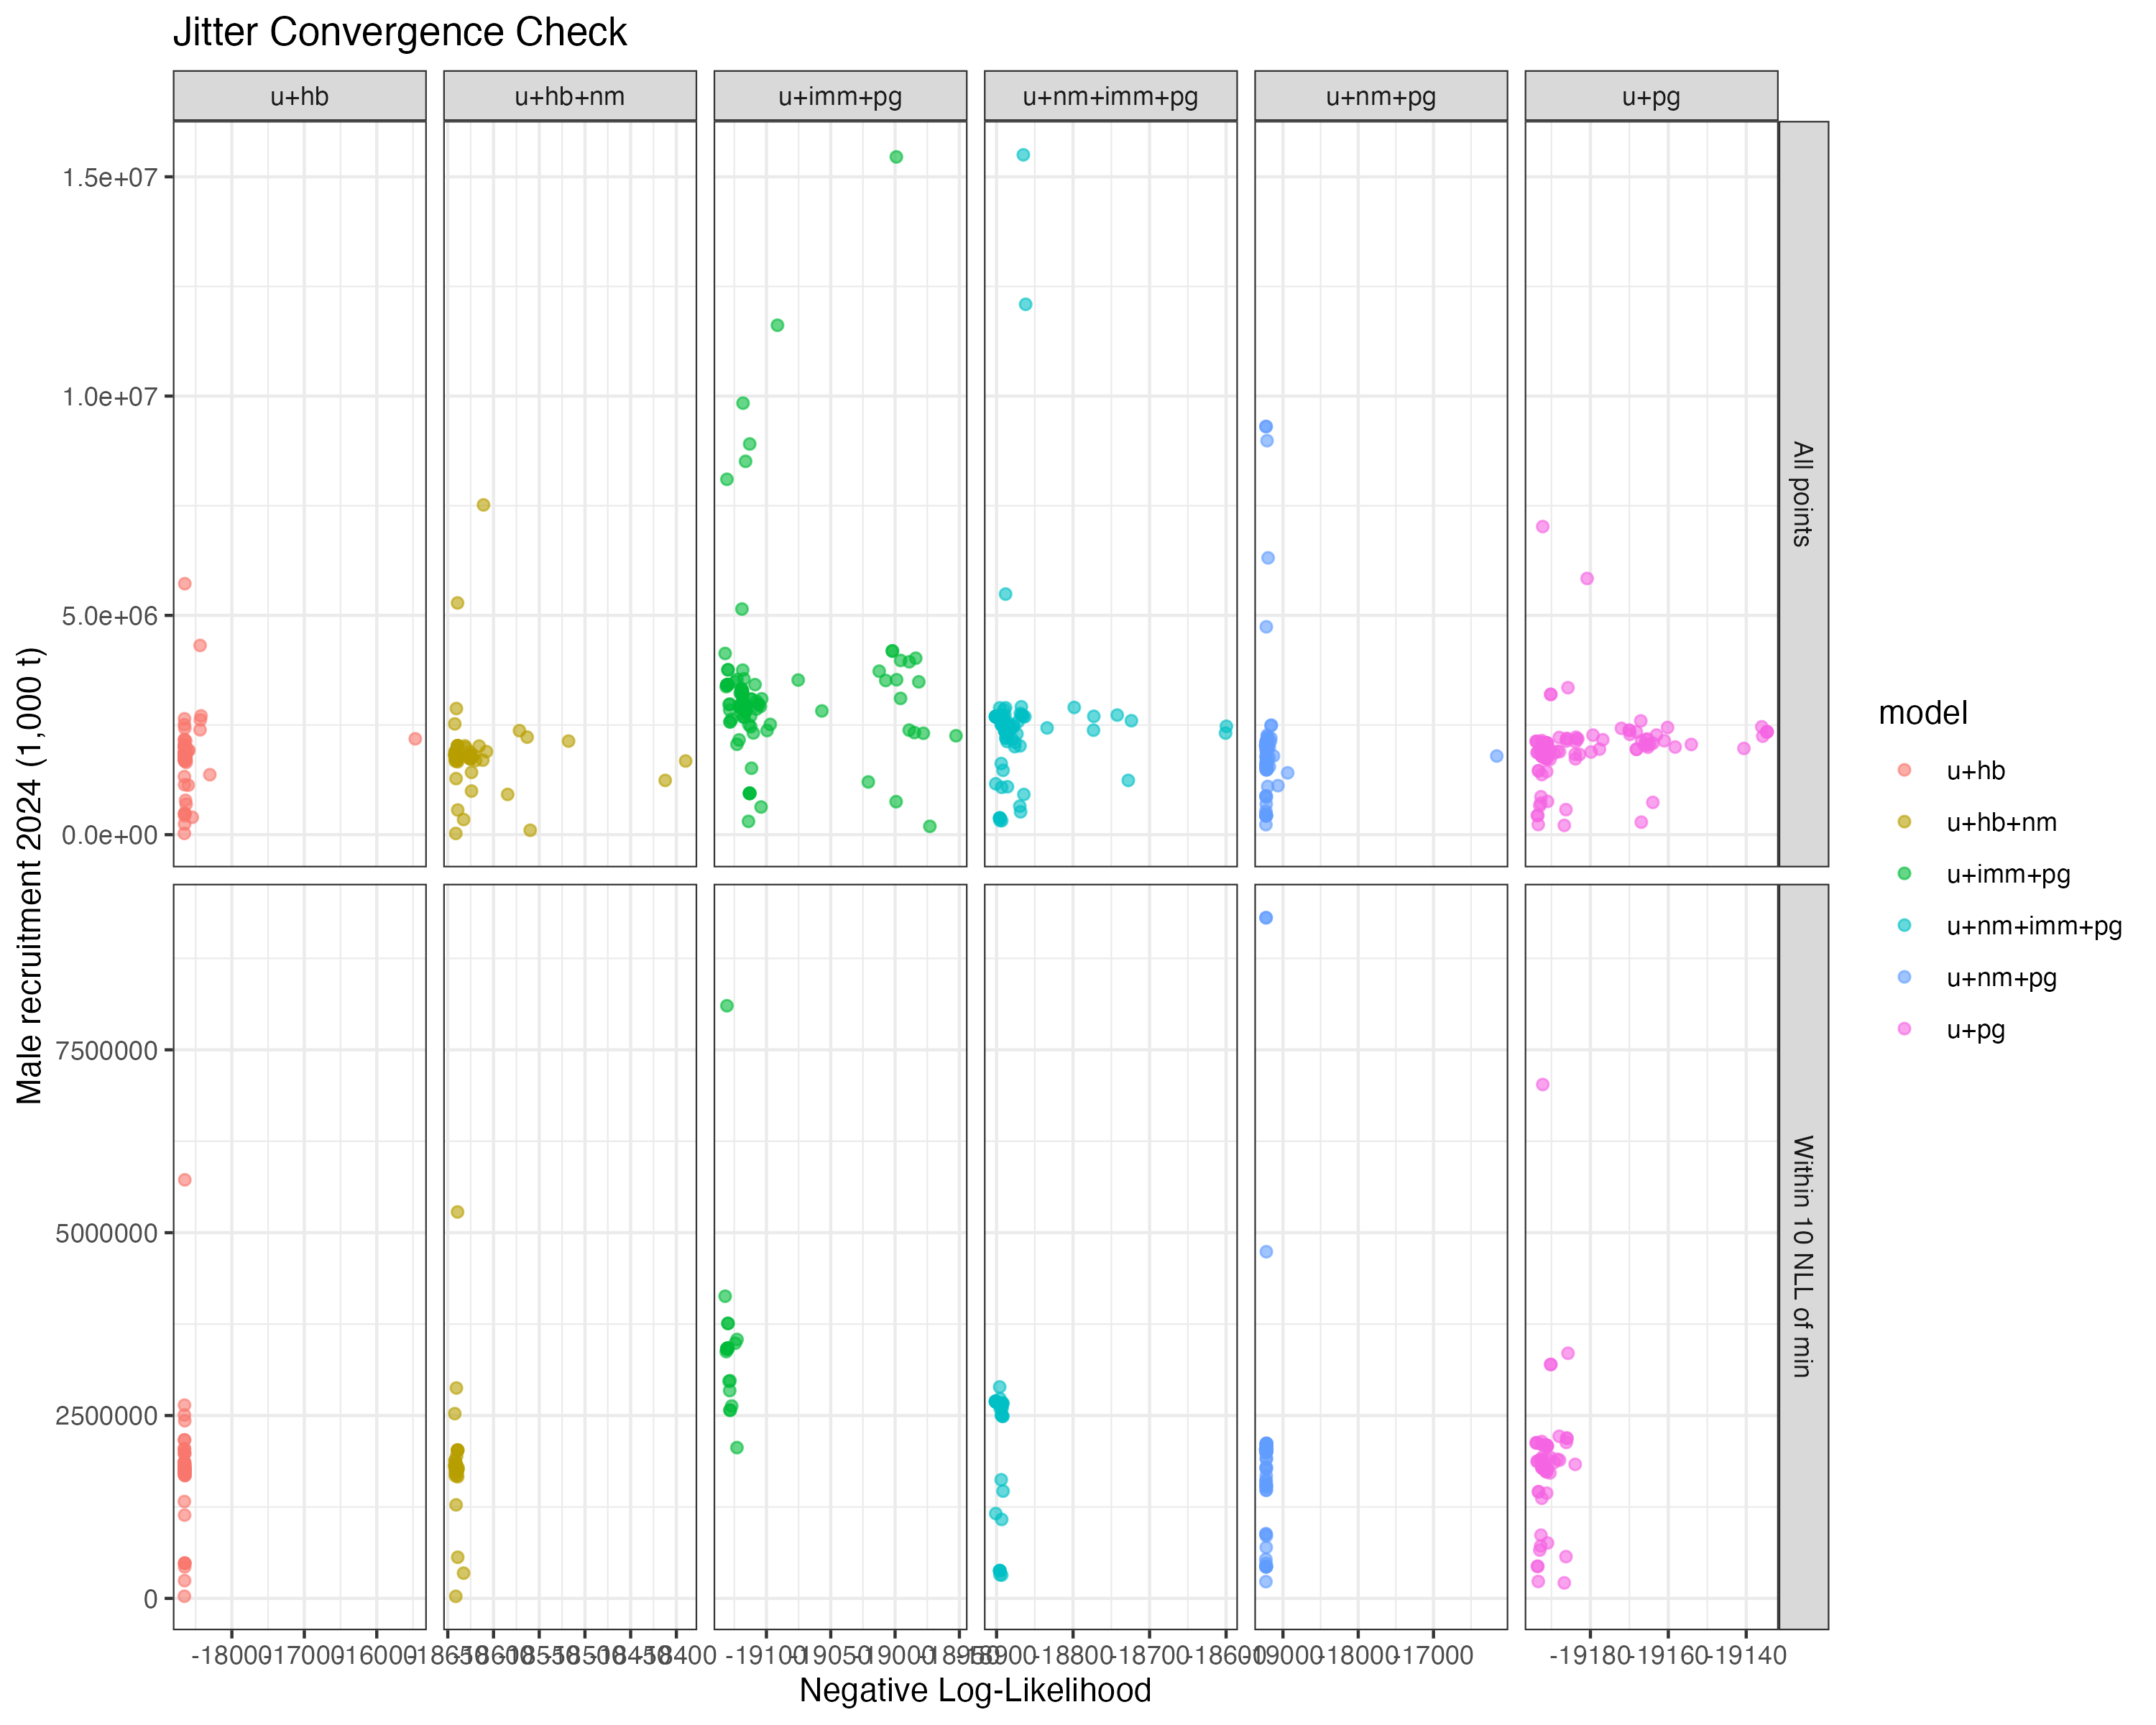
\includegraphics[width=1\linewidth]{plots/jittered_results_rec} \caption{Estimates of male recruitment in 2024 resulting from 100 jitter runs for the models that span the structural and data choices presented in this document. Each point is a converged jitter run; clouds separated vertically reflect alternative local optima.}\label{fig:jitt-rec}
\end{figure}

\newpage

\begin{figure}[H]
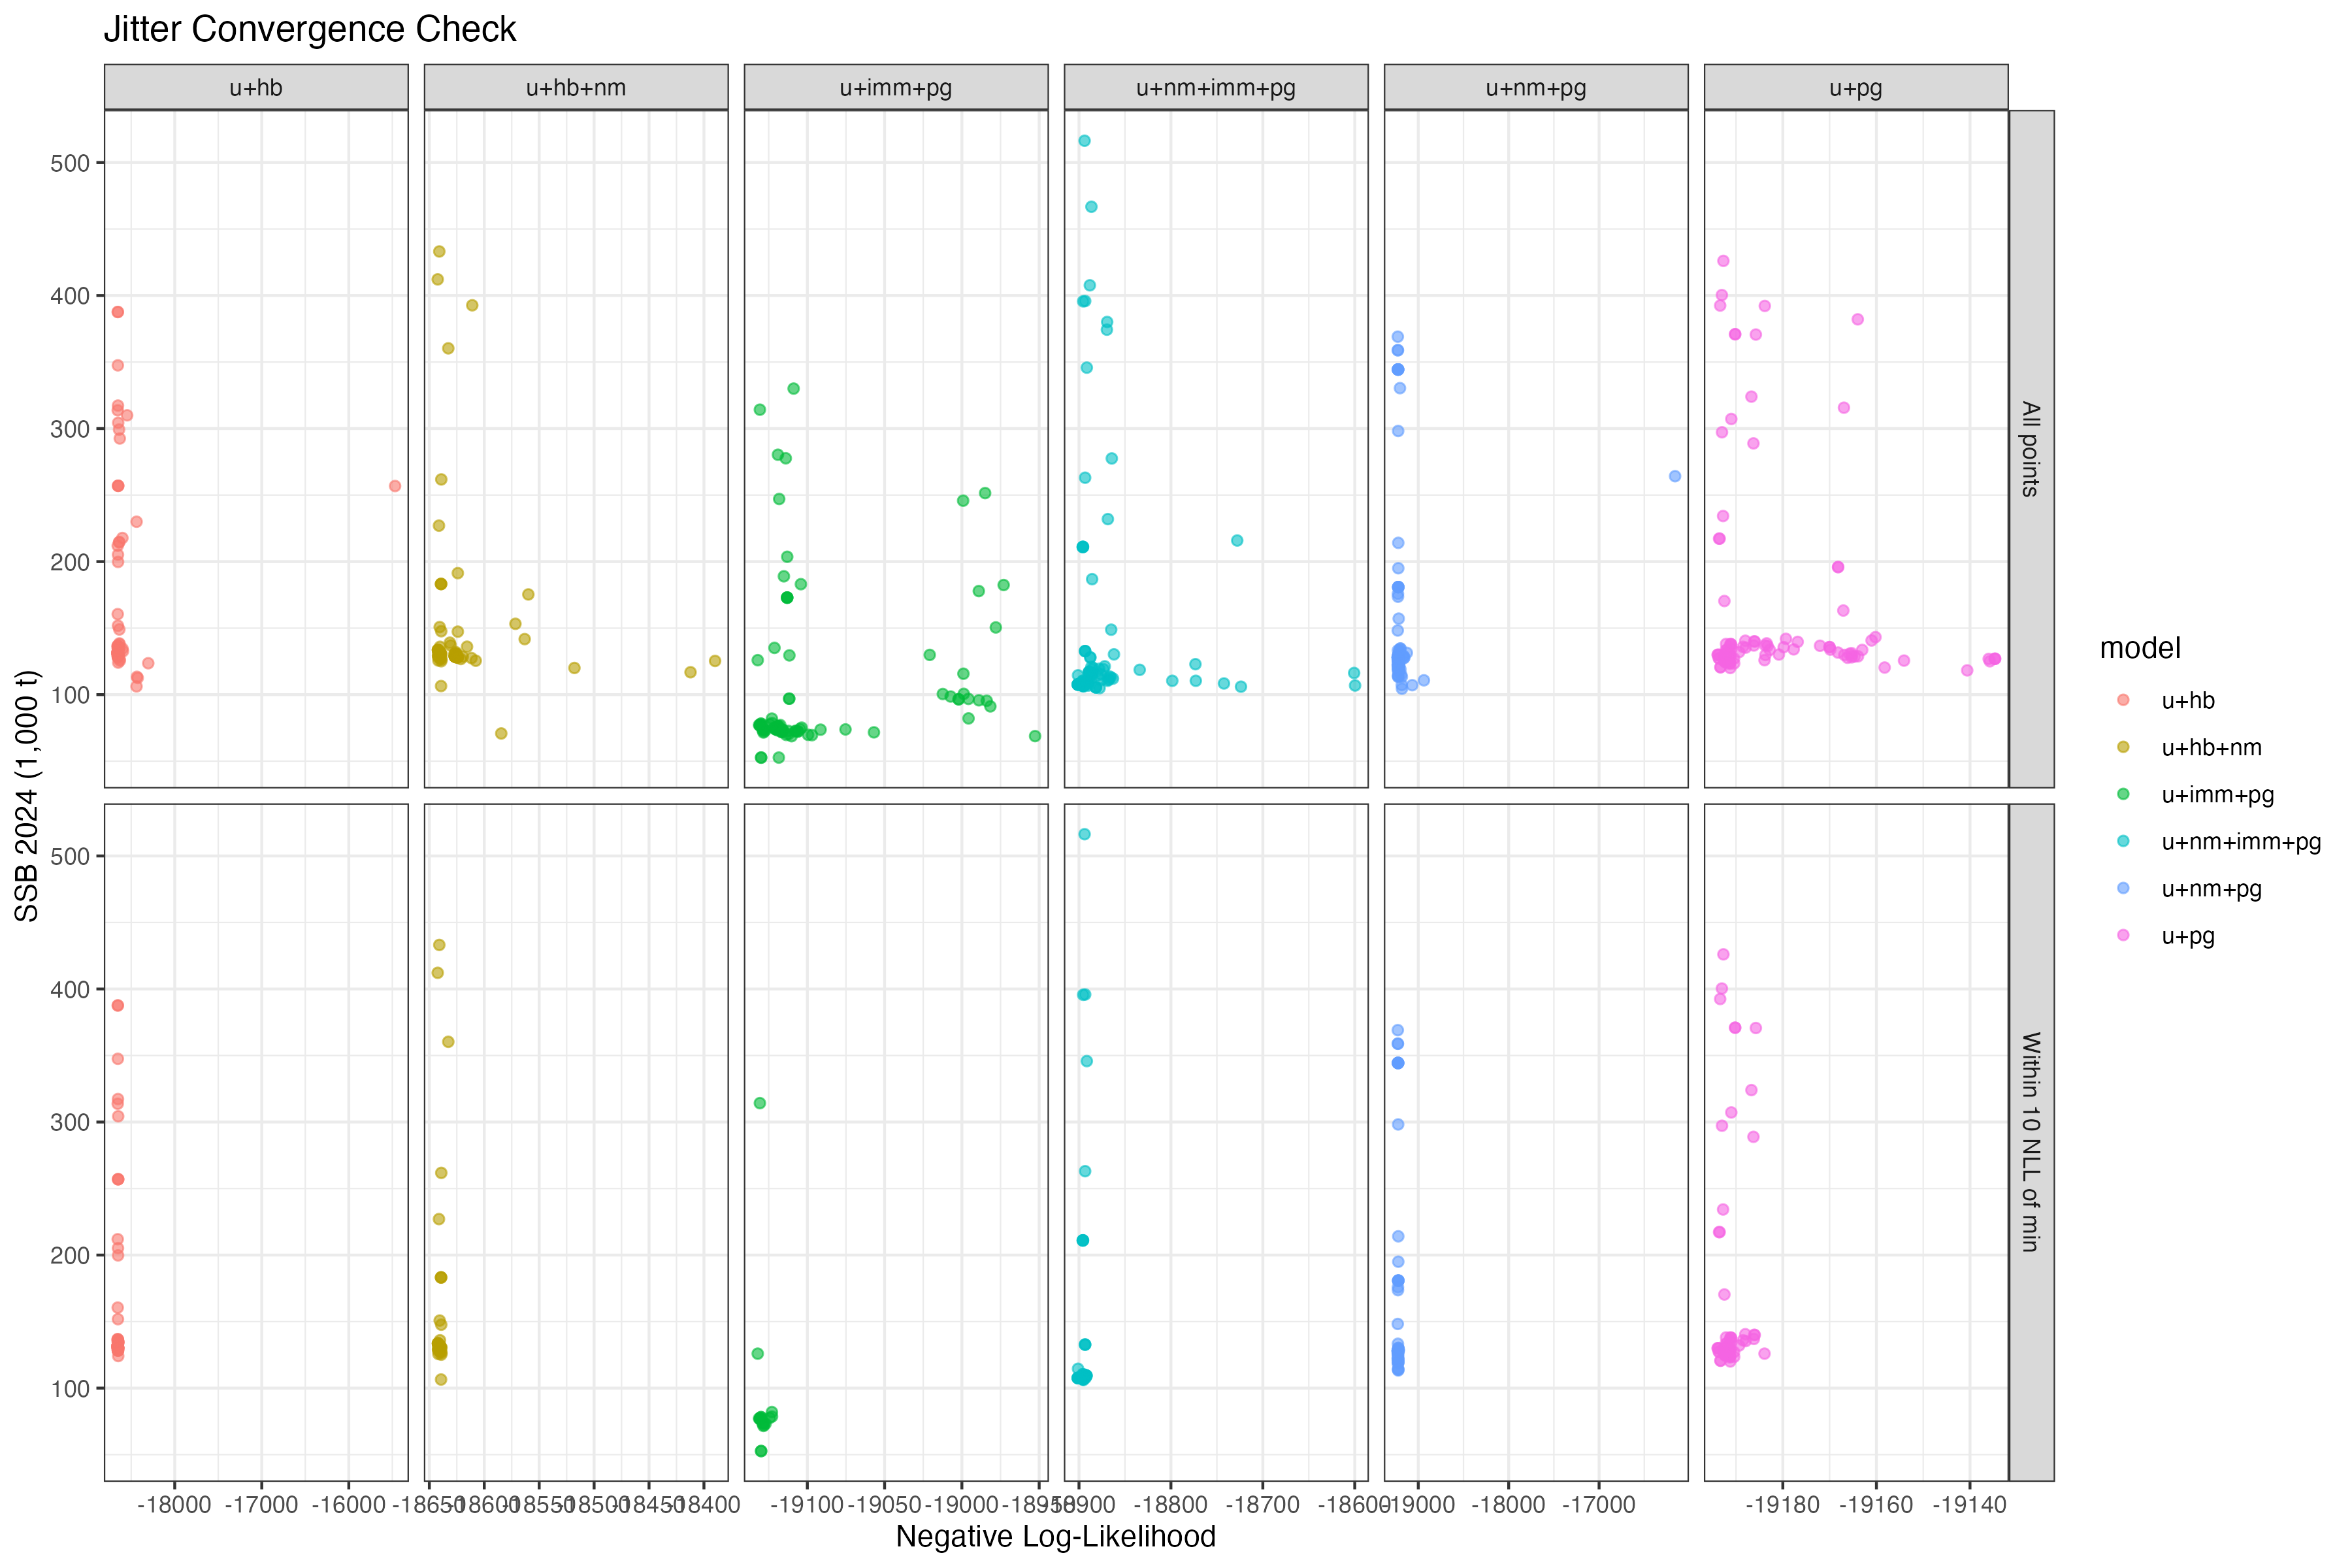
\includegraphics[width=1\linewidth]{plots/jittered_results_ssb} \caption{Estimates of MMB in 2024 resulting from 100 jitter runs for the models that span the structural and data choices presented in this document. Each point is a converged jitter run; clouds separated vertically reflect alternative local optima.}\label{fig:jitt-ssb}
\end{figure}

\newpage

\begin{landscape}
\begin{figure}[H]
\includegraphics[width=1\linewidth]{SAFE_snow_gmacs_files/figure-latex/mmbfits-1} \caption{Model fits to the observed mature biomass at survey.}\label{fig:mmbfits}
\end{figure}

\end{landscape}
\newpage

\begin{figure}[H]
\includegraphics[width=1\linewidth]{SAFE_snow_gmacs_files/figure-latex/growthfits-1} \caption{Model fits (colored lines) to the growth data (dots). Black dots are historical observations; red dots are new data for 2025.}\label{fig:growthfits}
\end{figure}

\newpage

\begin{figure}[H]
\includegraphics[width=1\linewidth]{SAFE_snow_gmacs_files/figure-latex/catchfits-1} \caption{Model fits to catch data.}\label{fig:catchfits}
\end{figure}

\newpage

\begin{figure}[H]
\includegraphics[width=1\linewidth]{SAFE_snow_gmacs_files/figure-latex/obs-101-vs-pred-1} \caption{Estimated biomass of male crab >101mm carapace width from the survey (black line and dots with gray 95th CI) and from each model in the assessment (colored lines).}\label{fig:obs-101-vs-pred}
\end{figure}

\newpage

\begin{figure}[H]
\includegraphics[width=1\linewidth]{SAFE_snow_gmacs_files/figure-latex/select-prior-1} \caption{Estimated survey selectivity (lines) with normal priors derived from BSFRF selectivity experiment data. Points are the mean of the prior at a given size; intervals are 95th quantiles based on input CVs.}\label{fig:select-prior}
\end{figure}

\newpage

\begin{figure}[H]
\includegraphics[width=1\linewidth]{SAFE_snow_gmacs_files/figure-latex/predselectfish-1} \caption{Estimated selectivities by fishing fleet and sex for capture and retained catches.}\label{fig:predselectfish}
\end{figure}

\newpage

\begin{figure}[H]
\includegraphics[width=1\linewidth]{SAFE_snow_gmacs_files/figure-latex/predfmort-1} \caption{Estimated fishing mortalities for the directed and non-directed fisheries.}\label{fig:predfmort}
\end{figure}

\newpage

\begin{figure}[H]
\includegraphics[width=1\linewidth]{SAFE_snow_gmacs_files/figure-latex/predmat-1} \caption{Estimated (black line) or specified (colored lines) probability(s) of maturing for male crab.}\label{fig:predmat}
\end{figure}

\newpage

\begin{figure}[H]
\includegraphics[width=1\linewidth]{SAFE_snow_gmacs_files/figure-latex/recruits-1} \caption{Estimated recruitment by sex (bottom) and proportions recruiting to length bin (top) by model.}\label{fig:recruits}
\end{figure}

\newpage

\begin{figure}[H]
\includegraphics[width=1\linewidth]{SAFE_snow_gmacs_files/figure-latex/nat-m-1} \caption{Estimated natural mortality by sex and maturity state. Natural mortality in all years previous to 2018 and after 2019 are equal to the estimated M in 2017.}\label{fig:nat-m}
\end{figure}

\newpage

\begin{figure}[H]
\includegraphics[width=1\linewidth]{SAFE_snow_gmacs_files/figure-latex/predmmb-1} \caption{Model predicted mature male biomass at mating time in 1,000 tonnes. Dashed horizontal lines are half of the respective BMSY proxies based on B35\% of a given management currency (i.e. MSST).}\label{fig:predmmb}
\end{figure}

\newpage

\section{Size composition fits}\label{size-composition-fits}

\begin{figure}
\centering
\pandocbounded{
\includegraphics[keepaspectratio]{SAFE_snow_gmacs_files/plots/size_comp_plot_1_NMFS_Trawl_1982_female_discarded_immature_New maturity.png}}
\caption{Model fits (lines) to size composition data (grey bars): NMFS Trawl 1982 female discarded immature New maturity.}
\end{figure}

\newpage

\begin{figure}
\centering
\pandocbounded{
\includegraphics[keepaspectratio]{SAFE_snow_gmacs_files/plots/size_comp_plot_2_NMFS_Trawl_1982_female_discarded_mature_New maturity.png}}
\caption{Model fits (lines) to size composition data (grey bars): NMFS Trawl 1982 female discarded mature New maturity.}
\end{figure}

\newpage

\begin{figure}
\centering
\pandocbounded{
\includegraphics[keepaspectratio]{SAFE_snow_gmacs_files/plots/size_comp_plot_3_NMFS_Trawl_1982_male_discarded_immature_New maturity.png}}
\caption{Model fits (lines) to size composition data (grey bars): NMFS Trawl 1982 male discarded immature New maturity.}
\end{figure}

\newpage

\begin{figure}
\centering
\pandocbounded{
\includegraphics[keepaspectratio]{SAFE_snow_gmacs_files/plots/size_comp_plot_4_NMFS_Trawl_1982_male_discarded_mature_New maturity.png}}
\caption{Model fits (lines) to size composition data (grey bars): NMFS Trawl 1982 male discarded mature New maturity.}
\end{figure}

\newpage

\begin{figure}
\centering
\pandocbounded{
\includegraphics[keepaspectratio]{SAFE_snow_gmacs_files/plots/size_comp_plot_5_NMFS_Trawl_1982_female_discarded_immature_Old maturity.png}}
\caption{Model fits (lines) to size composition data (grey bars): NMFS Trawl 1982 female discarded immature Old maturity.}
\end{figure}

\newpage

\begin{figure}
\centering
\pandocbounded{
\includegraphics[keepaspectratio]{SAFE_snow_gmacs_files/plots/size_comp_plot_6_NMFS_Trawl_1982_female_discarded_mature_Old maturity.png}}
\caption{Model fits (lines) to size composition data (grey bars): NMFS Trawl 1982 female discarded mature Old maturity.}
\end{figure}

\newpage

\begin{figure}
\centering
\pandocbounded{
\includegraphics[keepaspectratio]{SAFE_snow_gmacs_files/plots/size_comp_plot_7_NMFS_Trawl_1982_male_discarded_immature_Old maturity.png}}
\caption{Model fits (lines) to size composition data (grey bars): NMFS Trawl 1982 male discarded immature Old maturity.}
\end{figure}

\newpage

\begin{figure}
\centering
\pandocbounded{
\includegraphics[keepaspectratio]{SAFE_snow_gmacs_files/plots/size_comp_plot_8_NMFS_Trawl_1982_male_discarded_mature_Old maturity.png}}
\caption{Model fits (lines) to size composition data (grey bars): NMFS Trawl 1982 male discarded mature Old maturity.}
\end{figure}

\newpage

\begin{figure}
\centering
\pandocbounded{
\includegraphics[keepaspectratio]{SAFE_snow_gmacs_files/plots/size_comp_plot_9_NMFS_Trawl_1982_hybrid_female_discarded_immature_New maturity.png}}
\caption{Model fits (lines) to size composition data (grey bars): NMFS Trawl 1982 hybrid female discarded immature New maturity.}
\end{figure}

\newpage

\begin{figure}
\centering
\pandocbounded{
\includegraphics[keepaspectratio]{SAFE_snow_gmacs_files/plots/size_comp_plot_10_NMFS_Trawl_1982_hybrid_female_discarded_mature_New maturity.png}}
\caption{Model fits (lines) to size composition data (grey bars): NMFS Trawl 1982 hybrid female discarded mature New maturity.}
\end{figure}

\newpage

\begin{figure}
\centering
\pandocbounded{
\includegraphics[keepaspectratio]{SAFE_snow_gmacs_files/plots/size_comp_plot_11_NMFS_Trawl_1982_hybrid_male_discarded_immature_New maturity.png}}
\caption{Model fits (lines) to size composition data (grey bars): NMFS Trawl 1982 hybrid male discarded immature New maturity.}
\end{figure}

\newpage

\begin{figure}
\centering
\pandocbounded{
\includegraphics[keepaspectratio]{SAFE_snow_gmacs_files/plots/size_comp_plot_12_NMFS_Trawl_1982_hybrid_male_discarded_mature_New maturity.png}}
\caption{Model fits (lines) to size composition data (grey bars): NMFS Trawl 1982 hybrid male discarded mature New maturity.}
\end{figure}

\newpage

\begin{figure}
\centering
\pandocbounded{
\includegraphics[keepaspectratio]{SAFE_snow_gmacs_files/plots/size_comp_plot_13_NMFS_Trawl_1982_hybrid_female_discarded_immature_Old maturity.png}}
\caption{Model fits (lines) to size composition data (grey bars): NMFS Trawl 1982 hybrid female discarded immature Old maturity.}
\end{figure}

\newpage

\begin{figure}
\centering
\pandocbounded{
\includegraphics[keepaspectratio]{SAFE_snow_gmacs_files/plots/size_comp_plot_14_NMFS_Trawl_1982_hybrid_female_discarded_mature_Old maturity.png}}
\caption{Model fits (lines) to size composition data (grey bars): NMFS Trawl 1982 hybrid female discarded mature Old maturity.}
\end{figure}

\newpage

\begin{figure}
\centering
\pandocbounded{
\includegraphics[keepaspectratio]{SAFE_snow_gmacs_files/plots/size_comp_plot_15_NMFS_Trawl_1982_hybrid_male_discarded_immature_Old maturity.png}}
\caption{Model fits (lines) to size composition data (grey bars): NMFS Trawl 1982 hybrid male discarded immature Old maturity.}
\end{figure}

\newpage

\begin{figure}
\centering
\pandocbounded{
\includegraphics[keepaspectratio]{SAFE_snow_gmacs_files/plots/size_comp_plot_16_NMFS_Trawl_1982_hybrid_male_discarded_mature_Old maturity.png}}
\caption{Model fits (lines) to size composition data (grey bars): NMFS Trawl 1982 hybrid male discarded mature Old maturity.}
\end{figure}

\newpage

\begin{figure}
\centering
\pandocbounded{
\includegraphics[keepaspectratio]{SAFE_snow_gmacs_files/plots/size_comp_plot_17_NMFS_Trawl_1989_female_discarded_immature_New maturity.png}}
\caption{Model fits (lines) to size composition data (grey bars): NMFS Trawl 1989 female discarded immature New maturity.}
\end{figure}

\newpage

\begin{figure}
\centering
\pandocbounded{
\includegraphics[keepaspectratio]{SAFE_snow_gmacs_files/plots/size_comp_plot_18_NMFS_Trawl_1989_female_discarded_mature_New maturity.png}}
\caption{Model fits (lines) to size composition data (grey bars): NMFS Trawl 1989 female discarded mature New maturity.}
\end{figure}

\newpage

\begin{figure}
\centering
\pandocbounded{
\includegraphics[keepaspectratio]{SAFE_snow_gmacs_files/plots/size_comp_plot_19_NMFS_Trawl_1989_male_discarded_immature_New maturity.png}}
\caption{Model fits (lines) to size composition data (grey bars): NMFS Trawl 1989 male discarded immature New maturity.}
\end{figure}

\newpage

\begin{figure}
\centering
\pandocbounded{
\includegraphics[keepaspectratio]{SAFE_snow_gmacs_files/plots/size_comp_plot_20_NMFS_Trawl_1989_male_discarded_mature_New maturity.png}}
\caption{Model fits (lines) to size composition data (grey bars): NMFS Trawl 1989 male discarded mature New maturity.}
\end{figure}

\newpage

\begin{figure}
\centering
\pandocbounded{
\includegraphics[keepaspectratio]{SAFE_snow_gmacs_files/plots/size_comp_plot_21_NMFS_Trawl_1989_female_discarded_immature_Old maturity.png}}
\caption{Model fits (lines) to size composition data (grey bars): NMFS Trawl 1989 female discarded immature Old maturity.}
\end{figure}

\newpage

\begin{figure}
\centering
\pandocbounded{
\includegraphics[keepaspectratio]{SAFE_snow_gmacs_files/plots/size_comp_plot_22_NMFS_Trawl_1989_female_discarded_mature_Old maturity.png}}
\caption{Model fits (lines) to size composition data (grey bars): NMFS Trawl 1989 female discarded mature Old maturity.}
\end{figure}

\newpage

\begin{figure}
\centering
\pandocbounded{
\includegraphics[keepaspectratio]{SAFE_snow_gmacs_files/plots/size_comp_plot_23_NMFS_Trawl_1989_male_discarded_immature_Old maturity.png}}
\caption{Model fits (lines) to size composition data (grey bars): NMFS Trawl 1989 male discarded immature Old maturity.}
\end{figure}

\newpage

\begin{figure}
\centering
\pandocbounded{
\includegraphics[keepaspectratio]{SAFE_snow_gmacs_files/plots/size_comp_plot_24_NMFS_Trawl_1989_male_discarded_mature_Old maturity.png}}
\caption{Model fits (lines) to size composition data (grey bars): NMFS Trawl 1989 male discarded mature Old maturity.}
\end{figure}

\newpage

\begin{figure}
\centering
\pandocbounded{
\includegraphics[keepaspectratio]{SAFE_snow_gmacs_files/plots/size_comp_plot_25_NMFS_Trawl_1989_hybrid_female_discarded_immature_New maturity.png}}
\caption{Model fits (lines) to size composition data (grey bars): NMFS Trawl 1989 hybrid female discarded immature New maturity.}
\end{figure}

\newpage

\begin{figure}
\centering
\pandocbounded{
\includegraphics[keepaspectratio]{SAFE_snow_gmacs_files/plots/size_comp_plot_26_NMFS_Trawl_1989_hybrid_female_discarded_mature_New maturity.png}}
\caption{Model fits (lines) to size composition data (grey bars): NMFS Trawl 1989 hybrid female discarded mature New maturity.}
\end{figure}

\newpage

\begin{figure}
\centering
\pandocbounded{
\includegraphics[keepaspectratio]{SAFE_snow_gmacs_files/plots/size_comp_plot_27_NMFS_Trawl_1989_hybrid_male_discarded_immature_New maturity.png}}
\caption{Model fits (lines) to size composition data (grey bars): NMFS Trawl 1989 hybrid male discarded immature New maturity.}
\end{figure}

\newpage

\begin{figure}
\centering
\pandocbounded{
\includegraphics[keepaspectratio]{SAFE_snow_gmacs_files/plots/size_comp_plot_28_NMFS_Trawl_1989_hybrid_male_discarded_mature_New maturity.png}}
\caption{Model fits (lines) to size composition data (grey bars): NMFS Trawl 1989 hybrid male discarded mature New maturity.}
\end{figure}

\newpage

\begin{figure}
\centering
\pandocbounded{
\includegraphics[keepaspectratio]{SAFE_snow_gmacs_files/plots/size_comp_plot_29_NMFS_Trawl_1989_hybrid_female_discarded_immature_Old maturity.png}}
\caption{Model fits (lines) to size composition data (grey bars): NMFS Trawl 1989 hybrid female discarded immature Old maturity.}
\end{figure}

\newpage

\begin{figure}
\centering
\pandocbounded{
\includegraphics[keepaspectratio]{SAFE_snow_gmacs_files/plots/size_comp_plot_30_NMFS_Trawl_1989_hybrid_female_discarded_mature_Old maturity.png}}
\caption{Model fits (lines) to size composition data (grey bars): NMFS Trawl 1989 hybrid female discarded mature Old maturity.}
\end{figure}

\newpage

\begin{figure}
\centering
\pandocbounded{
\includegraphics[keepaspectratio]{SAFE_snow_gmacs_files/plots/size_comp_plot_31_NMFS_Trawl_1989_hybrid_male_discarded_immature_Old maturity.png}}
\caption{Model fits (lines) to size composition data (grey bars): NMFS Trawl 1989 hybrid male discarded immature Old maturity.}
\end{figure}

\newpage

\begin{figure}
\centering
\pandocbounded{
\includegraphics[keepaspectratio]{SAFE_snow_gmacs_files/plots/size_comp_plot_32_NMFS_Trawl_1989_hybrid_male_discarded_mature_Old maturity.png}}
\caption{Model fits (lines) to size composition data (grey bars): NMFS Trawl 1989 hybrid male discarded mature Old maturity.}
\end{figure}

\newpage

\begin{figure}
\centering
\pandocbounded{
\includegraphics[keepaspectratio]{SAFE_snow_gmacs_files/plots/size_comp_plot_33_Pot_Fishery_female_discarded_undetermined_New maturity.png}}
\caption{Model fits (lines) to size composition data (grey bars): Pot Fishery female discarded undetermined New maturity.}
\end{figure}

\newpage

\begin{figure}
\centering
\pandocbounded{
\includegraphics[keepaspectratio]{SAFE_snow_gmacs_files/plots/size_comp_plot_34_Pot_Fishery_male_retained_undetermined_New maturity.png}}
\caption{Model fits (lines) to size composition data (grey bars): Pot Fishery male retained undetermined New maturity.}
\end{figure}

\newpage

\begin{figure}
\centering
\pandocbounded{
\includegraphics[keepaspectratio]{SAFE_snow_gmacs_files/plots/size_comp_plot_35_Pot_Fishery_male_total_undetermined_New maturity.png}}
\caption{Model fits (lines) to size composition data (grey bars): Pot Fishery male total undetermined New maturity.}
\end{figure}

\newpage

\begin{figure}
\centering
\pandocbounded{
\includegraphics[keepaspectratio]{SAFE_snow_gmacs_files/plots/size_comp_plot_36_Pot_Fishery_female_discarded_undetermined_Old maturity.png}}
\caption{Model fits (lines) to size composition data (grey bars): Pot Fishery female discarded undetermined Old maturity.}
\end{figure}

\newpage

\begin{figure}
\centering
\pandocbounded{
\includegraphics[keepaspectratio]{SAFE_snow_gmacs_files/plots/size_comp_plot_37_Pot_Fishery_male_retained_undetermined_Old maturity.png}}
\caption{Model fits (lines) to size composition data (grey bars): Pot Fishery male retained undetermined Old maturity.}
\end{figure}

\newpage

\begin{figure}
\centering
\pandocbounded{
\includegraphics[keepaspectratio]{SAFE_snow_gmacs_files/plots/size_comp_plot_38_Pot_Fishery_male_total_undetermined_Old maturity.png}}
\caption{Model fits (lines) to size composition data (grey bars): Pot Fishery male total undetermined Old maturity.}
\end{figure}

\newpage

\begin{figure}
\centering
\pandocbounded{
\includegraphics[keepaspectratio]{SAFE_snow_gmacs_files/plots/size_comp_plot_39_Pot_fishery_compfix_female_discarded_undetermined_New maturity.png}}
\caption{Model fits (lines) to size composition data (grey bars): Pot fishery compfix female discarded undetermined New maturity.}
\end{figure}

\newpage

\begin{figure}
\centering
\pandocbounded{
\includegraphics[keepaspectratio]{SAFE_snow_gmacs_files/plots/size_comp_plot_40_Pot_fishery_compfix_male_retained_undetermined_New maturity.png}}
\caption{Model fits (lines) to size composition data (grey bars): Pot fishery compfix male retained undetermined New maturity.}
\end{figure}

\newpage

\begin{figure}
\centering
\pandocbounded{
\includegraphics[keepaspectratio]{SAFE_snow_gmacs_files/plots/size_comp_plot_41_Pot_fishery_compfix_male_total_undetermined_New maturity.png}}
\caption{Model fits (lines) to size composition data (grey bars): Pot fishery compfix male total undetermined New maturity.}
\end{figure}

\newpage

\begin{figure}
\centering
\pandocbounded{
\includegraphics[keepaspectratio]{SAFE_snow_gmacs_files/plots/size_comp_plot_42_Pot_fishery_compfix_female_discarded_undetermined_Old maturity.png}}
\caption{Model fits (lines) to size composition data (grey bars): Pot fishery compfix female discarded undetermined Old maturity.}
\end{figure}

\newpage

\begin{figure}
\centering
\pandocbounded{
\includegraphics[keepaspectratio]{SAFE_snow_gmacs_files/plots/size_comp_plot_43_Pot_fishery_compfix_male_retained_undetermined_Old maturity.png}}
\caption{Model fits (lines) to size composition data (grey bars): Pot fishery compfix male retained undetermined Old maturity.}
\end{figure}

\newpage

\begin{figure}
\centering
\pandocbounded{
\includegraphics[keepaspectratio]{SAFE_snow_gmacs_files/plots/size_comp_plot_44_Pot_fishery_compfix_male_total_undetermined_Old maturity.png}}
\caption{Model fits (lines) to size composition data (grey bars): Pot fishery compfix male total undetermined Old maturity.}
\end{figure}

\newpage

\begin{figure}
\centering
\pandocbounded{
\includegraphics[keepaspectratio]{SAFE_snow_gmacs_files/plots/size_comp_plot_45_Pot_fishery_hybrid_female_discarded_undetermined_New maturity.png}}
\caption{Model fits (lines) to size composition data (grey bars): Pot fishery hybrid female discarded undetermined New maturity.}
\end{figure}

\newpage

\begin{figure}
\centering
\pandocbounded{
\includegraphics[keepaspectratio]{SAFE_snow_gmacs_files/plots/size_comp_plot_46_Pot_fishery_hybrid_male_retained_undetermined_New maturity.png}}
\caption{Model fits (lines) to size composition data (grey bars): Pot fishery hybrid male retained undetermined New maturity.}
\end{figure}

\newpage

\begin{figure}
\centering
\pandocbounded{
\includegraphics[keepaspectratio]{SAFE_snow_gmacs_files/plots/size_comp_plot_47_Pot_fishery_hybrid_male_total_undetermined_New maturity.png}}
\caption{Model fits (lines) to size composition data (grey bars): Pot fishery hybrid male total undetermined New maturity.}
\end{figure}

\newpage

\begin{figure}
\centering
\pandocbounded{
\includegraphics[keepaspectratio]{SAFE_snow_gmacs_files/plots/size_comp_plot_48_Pot_fishery_hybrid_female_discarded_undetermined_Old maturity.png}}
\caption{Model fits (lines) to size composition data (grey bars): Pot fishery hybrid female discarded undetermined Old maturity.}
\end{figure}

\newpage

\begin{figure}
\centering
\pandocbounded{
\includegraphics[keepaspectratio]{SAFE_snow_gmacs_files/plots/size_comp_plot_49_Pot_fishery_hybrid_male_retained_undetermined_Old maturity.png}}
\caption{Model fits (lines) to size composition data (grey bars): Pot fishery hybrid male retained undetermined Old maturity.}
\end{figure}

\newpage

\begin{figure}
\centering
\pandocbounded{
\includegraphics[keepaspectratio]{SAFE_snow_gmacs_files/plots/size_comp_plot_50_Pot_fishery_hybrid_male_total_undetermined_Old maturity.png}}
\caption{Model fits (lines) to size composition data (grey bars): Pot fishery hybrid male total undetermined Old maturity.}
\end{figure}

\newpage

\begin{figure}
\centering
\pandocbounded{
\includegraphics[keepaspectratio]{SAFE_snow_gmacs_files/plots/size_comp_plot_51_Pot_fishery_plus_group_female_discarded_undetermined_New maturity.png}}
\caption{Model fits (lines) to size composition data (grey bars): Pot fishery plus group female discarded undetermined New maturity.}
\end{figure}

\newpage

\begin{figure}
\centering
\pandocbounded{
\includegraphics[keepaspectratio]{SAFE_snow_gmacs_files/plots/size_comp_plot_52_Pot_fishery_plus_group_male_retained_undetermined_New maturity.png}}
\caption{Model fits (lines) to size composition data (grey bars): Pot fishery plus group male retained undetermined New maturity.}
\end{figure}

\newpage

\begin{figure}
\centering
\pandocbounded{
\includegraphics[keepaspectratio]{SAFE_snow_gmacs_files/plots/size_comp_plot_53_Pot_fishery_plus_group_male_total_undetermined_New maturity.png}}
\caption{Model fits (lines) to size composition data (grey bars): Pot fishery plus group male total undetermined New maturity.}
\end{figure}

\newpage

\begin{figure}
\centering
\pandocbounded{
\includegraphics[keepaspectratio]{SAFE_snow_gmacs_files/plots/size_comp_plot_54_Pot_fishery_plus_group_female_discarded_undetermined_Old maturity.png}}
\caption{Model fits (lines) to size composition data (grey bars): Pot fishery plus group female discarded undetermined Old maturity.}
\end{figure}

\newpage

\begin{figure}
\centering
\pandocbounded{
\includegraphics[keepaspectratio]{SAFE_snow_gmacs_files/plots/size_comp_plot_55_Pot_fishery_plus_group_male_retained_undetermined_Old maturity.png}}
\caption{Model fits (lines) to size composition data (grey bars): Pot fishery plus group male retained undetermined Old maturity.}
\end{figure}

\newpage

\begin{figure}
\centering
\pandocbounded{
\includegraphics[keepaspectratio]{SAFE_snow_gmacs_files/plots/size_comp_plot_56_Pot_fishery_plus_group_male_total_undetermined_Old maturity.png}}
\caption{Model fits (lines) to size composition data (grey bars): Pot fishery plus group male total undetermined Old maturity.}
\end{figure}

\newpage

\begin{figure}
\centering
\pandocbounded{
\includegraphics[keepaspectratio]{SAFE_snow_gmacs_files/plots/size_comp_plot_57_Trawl_Bycatch_female_discarded_undetermined_New maturity.png}}
\caption{Model fits (lines) to size composition data (grey bars): Trawl Bycatch female discarded undetermined New maturity.}
\end{figure}

\newpage

\begin{figure}
\centering
\pandocbounded{
\includegraphics[keepaspectratio]{SAFE_snow_gmacs_files/plots/size_comp_plot_58_Trawl_Bycatch_male_discarded_undetermined_New maturity.png}}
\caption{Model fits (lines) to size composition data (grey bars): Trawl Bycatch male discarded undetermined New maturity.}
\end{figure}

\newpage

\begin{figure}
\centering
\pandocbounded{
\includegraphics[keepaspectratio]{SAFE_snow_gmacs_files/plots/size_comp_plot_59_Trawl_Bycatch_female_discarded_undetermined_Old maturity.png}}
\caption{Model fits (lines) to size composition data (grey bars): Trawl Bycatch female discarded undetermined Old maturity.}
\end{figure}

\newpage

\begin{figure}
\centering
\pandocbounded{
\includegraphics[keepaspectratio]{SAFE_snow_gmacs_files/plots/size_comp_plot_60_Trawl_Bycatch_male_discarded_undetermined_Old maturity.png}}
\caption{Model fits (lines) to size composition data (grey bars): Trawl Bycatch male discarded undetermined Old maturity.}
\end{figure}

\newpage

\end{document}
